%%%%%%%%%%%%%%%%%%%%%%%%%%%%%%%%%%%%%%%%%
% Tufte-Style Book (Minimal Template)
% LaTeX Template
% Version 1.0 (5/1/13)
%
% This template has been downloaded from:
% http://www.LaTeXTemplates.com
%
% License:
% CC BY-NC-SA 3.0 (http://creativecommons.org/licenses/by-nc-sa/3.0/)
%
% IMPORTANT NOTE:
% In addition to running BibTeX to compile the reference list from the .bib
% file, you will need to run MakeIndex to compile the index at the end of the
% document.
%
%%%%%%%%%%%%%%%%%%%%%%%%%%%%%%%%%%%%%%%%%

%----------------------------------------------------------------------------------------
%	PACKAGES AND OTHER DOCUMENT CONFIGURATIONS
%----------------------------------------------------------------------------------------

\documentclass{tufte-book} % Use the tufte-book class which in turn uses the tufte-common class

\hypersetup{colorlinks} % Comment this line if you don't wish to have colored links

\usepackage{microtype} % Improves character and word spacing

\usepackage{lipsum} % Inserts dummy text

\usepackage{booktabs} % Better horizontal rules in tables

\usepackage{graphicx} % Needed to insert images into the document
\graphicspath{{/Users/bapu/Projects/earth/writing/1-cooperation-textbook/images/}} % Sets the default location of pictures
\setkeys{Gin}{width=\linewidth,totalheight=\textheight,keepaspectratio} % Improves figure scaling

\usepackage{fancyvrb} % Allows customization of verbatim environments
\fvset{fontsize=\normalsize} % The font size of all verbatim text can be changed here

\newcommand{\hangp}[1]{\makebox[0pt][r]{(}#1\makebox[0pt][l]{)}} % New command to create parentheses around text in tables which take up no horizontal space - this improves column spacing
\newcommand{\hangstar}{\makebox[0pt][l]{*}} % New command to create asterisks in tables which take up no horizontal space - this improves column spacing

\usepackage{xspace} % Used for printing a trailing space better than using a tilde (~) using the \xspace command

\usepackage{amsmath}
\usepackage{tcolorbox}

\newcommand{\monthyear}{\ifcase\month\or January\or February\or March\or April\or May\or June\or July\or August\or September\or October\or November\or December\fi\space\number\year} % A command to print the current month and year

\newcommand{\openepigraph}[2]{ % This block sets up a command for printing an epigraph with 2 arguments - the quote and the author
\begin{fullwidth}
\sffamily\large
\begin{doublespace}
\noindent\allcaps{#1}\\ % The quote
\noindent\allcaps{#2} % The author
\end{doublespace}
\end{fullwidth}
}

\newcommand{\blankpage}{\newpage\hbox{}\thispagestyle{empty}\newpage} % Command to insert a blank page

\usepackage{makeidx} % Used to generate the index
\makeindex % Generate the index which is printed at the end of the document

%----------------------------------------------------------------------------------------
%	BOOK META-INFORMATION
%----------------------------------------------------------------------------------------

\title[Cooperation in Biological and Social Systems]{\par Cooperation in \par Biological and \par Social Systems} % Title of the book

\author{Bapu Vaitla} % Author

\publisher{Elsevier} % Publisher

%----------------------------------------------------------------------------------------

\begin{document}

\frontmatter

%----------------------------------------------------------------------------------------
%	EPIGRAPH
%----------------------------------------------------------------------------------------

\thispagestyle{empty}
\openepigraph{\textbf{Evolution is a light which illuminates all facts, a curve that all lines must follow.}}{Pierre Teilhard de Chardin, {\itshape The Phenomenon of Man, 1955}}


%----------------------------------------------------------------------------------------

\maketitle % Print the title page

%----------------------------------------------------------------------------------------
%	COPYRIGHT PAGE
%----------------------------------------------------------------------------------------

\newpage
\begin{fullwidth}
~\vfill
\thispagestyle{empty}
\setlength{\parindent}{0pt}
\setlength{\parskip}{\baselineskip}
Copyright \copyright\ \the\year\ \thanklessauthor

\par\smallcaps{Published by \thanklesspublisher}

\par\smallcaps{\url{http://www.bookwebsite.com}}

\par License information.\index{license}

\par\textit{First printing, \monthyear}
\end{fullwidth}

%----------------------------------------------------------------------------------------

\tableofcontents % Print the table of contents

%----------------------------------------------------------------------------------------

\listoffigures % Print a list of figures

%----------------------------------------------------------------------------------------

\listoftables % Print a list of tables

%----------------------------------------------------------------------------------------
%	DEDICATION PAGE
%----------------------------------------------------------------------------------------

\cleardoublepage
~\vfill
\begin{doublespace}
\noindent\fontsize{18}{22}\selectfont\itshape
\nohyphenation
Dedicated to my family and friends.
\end{doublespace}
\vfill
\vfill

%----------------------------------------------------------------------------------------
%	INTRODUCTION
%----------------------------------------------------------------------------------------

\cleardoublepage
\chapter{Introduction} 

Evolutionary history is a series of cooperative transitions. Life originated when free molecules aggregated within a membrane-bound, replicating, metabolizing cell. These independent replicators, grouped into chromosomes, formed a genomic partnership. Eukaryotic life arose from the fusion of two kinds of single-celled creatures, a host archeon species and the bacterial ancestor of mitochondria (and later, a further merging event with the ancestor of chloroplasts). Instead of clonally replicating, individual organisms mixed their genomes with other individuals in the process of sexual reproduction. Cells divided labor within multicellular bodies. Some organisms, both unicellular and multicellular, formed societies of cooperating individuals. Nearly all % true? 
species developed mutualistic relationships with other species, exchanging resources and protection. % among what else? 
In all of these cases, formerly independent replicating units became, over time, a single unit replicating together--the phenotypic target of natural selection. 

The history of \emph{Homo sapiens} follows a similar trajectory. Hominids % check whether should be different term
have been social for millions of years, tracing back to at least \emph{Australopethicus afarensis}, a species that existed 3.8 million years ago; the famous `' footprints %more here on them
hint at group living. Until about 10,000 years ago, however, human groups were restricted to small bands of no more than % number
people. In the millennia since, \emph{Homo sapiens} have built increasingly complex economic and political systems, with the majority of humanity transitioning through band, tribal, and chiefdom-based social structures to the nation-states of the modern world.\cite{service1971primitive} The stability and power of these systems depends on cooperation. Cooperative societies are those with well-functioning markets, efficient public institutions, and cultural norms well-adapted to environmental and economic challenges--all of which are enabling conditions for the cultural ideas and technologies that have fueled improvements in human well-being over the centuries. All of human history is in a sense a slow resolution of what social scientists call `the collective action problem': the search for incentives and ideas that encourage cooperation and constrain conflict.

Competition and conflict, however, are omnipresent in both non-human nature and human society. In biological systems, the pressures of natural selection at the lower level--i.e., the formerly independent unit--constantly threatens the integrity of the higher-level cooperative unit. The same is true of human systems: people cheat on their spouses, endangering the cooperative pair bond; we commit crimes against others, challenging social norms; we fail to pay taxes, weakening the state. In both biological and social systems, cooperation depends on mechanisms to monitor, sanction, and mitigate cheating. 

This book is an exploration of the tension between cooperation and conflict in nature. This tension lies at the heart of both evolutionary and ethical questions, and for this reason cooperation is an important concept in a wide range of sciences, including biochemistry, genetics, cellular biology, animal behavior, ecology, anthropology, sociology, economics, political science, and cognitive science. Each discipline defines the concept differently, but the core meaning--separate entities working together for mutual benefit--is consistent across fields. 

\section{Organization of the book}

\newthought{Chapter \ref{ch:framework}} provides an evolutionary and conceptual framework for the content that follows. It reviews the key concepts of evolution by natural selection, and then turns to the key theories of cooperation in the biological and social sciences, respectively: Hamilton's rule and the theory of collective action. The former offers a simple framework for understanding the conditions under which biological cooperation will emerge and stabilize--in short, when the benefit to a replicating entity and its genetic relatives (``inclusive fitness'') exceeds the cost to the same. The theory of collective action offers a similar exposition of the conditions that lead to stability of human cooperation. The purpose of this chapter is  to provide students with the analytic tools needed to understand both biological and social cooperation.

Chapters \ref{ch:origins}-\ref{ch:multicell} then look at the various levels of cooperation involved in the evolutionary transitions from molecules to individual. Chapter \ref{ch:origins} examines the leading hypotheses around the origins of life: how a collection of inorganic molecules created an auto-catalytic cycle--a process of metabolism and replication--within a cellular boundary, and highlights the challenges that such an innovation would have had to overcome. The cooperative schema between nucleic acids and proteins is a key feature of this new cooperative system. Chapter \ref{ch:genome} then describes the various kinds of cooperation that take place on the genome--a collection of informational molecules, each with their own urge to replicate, that nevertheless work together to optimize the chances for the genome as a whole to be copied into the next generation. The chapter also discusses various forms of `cheating' on the genome, including meiotic drive and the transposable elements that compose much of the total content of modern eukaryotic genomes. Chapter \ref{ch:endosymbiosis} recounts the stories of two remarkable, and possibly very unlikely, events in evolutionary history: the integration of mitochondrial and plastid elements within the cell, the eukaryotic design that all complex life on Earth shares. The chapter explores how these partnerships internal to the cell--to this day still possessing two separate genomes--may have remained stable in the face of internal selection pressures. Chapter \ref{ch:multicell} then discusses cooperation across cells: the invention of multicellularity. The chapter recounts the probable origin of multicellularity in colonial organisms and analyzes the mechanisms that coordinate function across specialized cells in modern organisms and prevent (in all but the rarest of cases) conflict within the body.

Chapters \ref{ch:sex}-\ref{ch:mutualism} look at transitions from individual to social life. Chapter \ref{ch:sex} discusses the various hypothesis put forward to explain the emergence of sex, a puzzling question given that clonal organisms replicate their entire genome while sexual organisms only replicate half--the ``twofold cost of sex''. Sexual partnerships, whether brief or protracted, are an excellent example of the continual tension between cooperation and competition in biology; each individual seeks to optimize their inclusive fitness, which sometimes leads to coordinated action and other times to cheating. Chapter \ref{ch:parenting} examines parenting, the cooperative care of children. Parenting is the set of behaviors that some species exhibit to ensure that their replicated genome optimizes its chances for survival in the initial stages of life. The field of parent-offspring conflict--the ways in which parents and children compete for resources, and the consequences of such conflict--has greatly illuminated our understanding of inclusive fitness. Chapter \ref{ch:eusociality} looks at species that are `eusocial,' i.e., that are characterized by cooperative care of offspring, a diverse age structure within the same colony, and a division of labor between reproductive and worker individuals. There is only a small number of eusocial species on Earth, but they nevertheless dominate many living systems; the social insects--ants, bees, wasps, and termites--are the most well-known, though a few examples exist in animals. Chapter \ref{ch:coord-recip} discusses cooperation between unrelated individuals. Behaviors like group hunting, grooming and cleaning, alarm calls, and food sharing can produce reciprocal benefits in social species. Such behaviors are, however, also vulnerable to difficult-to-detect cheating. Chapter \ref{ch:mutualism} is a snapshot of the many mutualistic relationships between species. The chapter focuses on two ubiquitous of tremendous ecological importance: plant-pollinator interactions and plant-mycorrhizal networks. The latter has been a particularly rich experimental ground for the study of cheating and sanctions.

Chapters \ref{ch:social-coop}-\ref{ch:intl-coop} focus on human systems. Chapter \ref{ch:social-coop} is a survey of the evolution of human social norms around cooperation. The chapter looks at institutions each of the four historical levels of social organization: bands, tribes, chiefdoms, and states. Norms around marriage and familial units are also covered, with an in-depth discussion of intrahousehold bargaining theory. The chapter concludes with a discussion of modern digital social networks, and how datasets from these networks can shed light on the cultural evolution of cooperation. Chapter \ref{ch:econ-coop} introduces the notion of trade as a form of cooperation--a voluntary exchange of goods that, in a hypothetical ideal scenario, yields desirable outcomes for all market players. The tension between competition and cooperation under the theory of efficient markets is examined, with a critical analysis of the conditions under which adverse outcomes, especially social inequality and negative environmental externalities, occur. Chapter \ref{ch:poli-coop} is an examination of the key ideas and institutions behind modern systems of political cooperation. The survey begins with a look at classical and modern democratic systems, including the rise of social contract theory in the past few centuries. The chapter also analyzes some of the critical unresolved problems around the design of voting and representation systems, and the types of pressures to which democratic institutions are subjected. Chapter \ref{ch:intl-coop} concludes the book by applying the concepts and tools students have learned in previous chapters to a series of in-depth case studies of current global collective action problems, including climate change, cyberterrorism, and infectious disease. The chapter examines the structure of institutions that confront these problems at various social levels--the family, the community, subnational governments, national governments, and international agencies—-with an analysis of the determinants of cooperation within and across levels. 

\section{Organization of each chapter}

\newthought{Each chapter} begins with a brief synopsis of its content. Section headings divide chapters into key themes, typically between three to five per chapter. References, figures, images, and tables are provided in the margin of each page for easy reference. Each chapter concludes with a list of key terms, suggestions for further reading, and study questions. The first use of key terms in the book appears in bold. These terms are essential to understanding the content of the book, and students are encouraged to review them in detail. A glossary at the end of the book defines all the key terms. 
All of the works cited in the main text are included in the bibliography at the end of the book. If the reader wishes to learn more in depth about the material in a given chapter, suggestions for further reading are given at the end of that chapter, with a brief description of the context of each text. *Starred texts are especially valuable. 

The study questions at the end of each chapter are divided into two categories: practice problems to hone skills, for which the answers are provided at www.[answers].edu, and topics to fuel classroom discussion. These latter questions do not have `right' or `wrong' answers, but rather are meant to encourage critical thinking in students.

%------------------------------------------------

% EXAMPLES OF FIGURES, MARGIN NOTES, AND TABLES

% \begin{marginfigure}
% 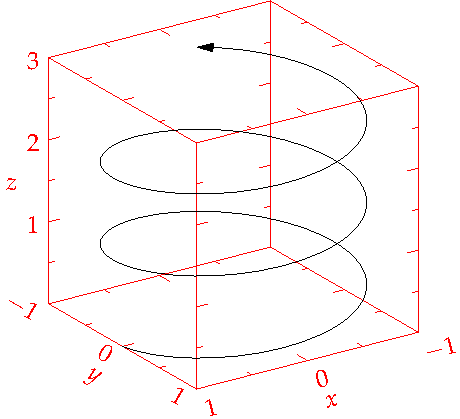
\includegraphics[width=\linewidth]{helix}
% \caption{This is a margin figure. }
% \label{fig:marginfig}
% \end{marginfigure}


% \begin{figure*}[h]
% 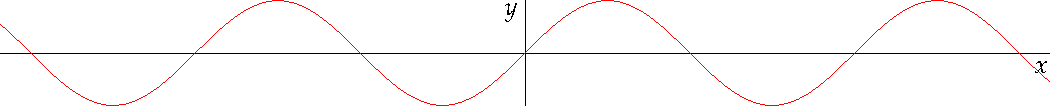
\includegraphics[width=\linewidth]{sine.pdf}
% \caption{This graph shows $y = \sin x$ from about $x = [-10, 10]$.
% \emph{Notice that this figure takes up the full page width.}}
% \label{fig:fullfig}
% \end{figure*}

% \marginnote{This is a random margin note. Notice that there isn't a number preceding the note, and there is no number in the main text where this note was written. Use \texttt{sidenote} to use a number.}

% \begin{table} % Add the following just after the closing bracket on this line to specify a position for the table on the page: [h], [t], [b] or [p] - these mean: here, top, bottom and on a separate page, respectively
% \centering % Centers the table on the page, comment out to left-justify
% \begin{tabular}{l c c c c c} % The final bracket specifies the number of columns in the table along with left and right borders which are specified using vertical bars (|); each column can be left, right or center-justified using l, r or c. To specify a precise width, use p{width}, e.g. p{5cm}
% \toprule % Top horizontal line
% & \multicolumn{5}{c}{Growth Media} \\ % Amalgamating several columns into one cell is done using the \multicolumn command as seen on this line
% \cmidrule(l){2-6} % Horizontal line spanning less than the full width of the table - you can add (r) or (l) just before the opening curly bracket to shorten the rule on the left or right side
% Strain & 1 & 2 & 3 & 4 & 5\\ % Column names row
% \midrule % In-table horizontal line
% GDS1002 & 0.962 & 0.821 & 0.356 & 0.682 & 0.801\\ % Content row 1
% NWN652 & 0.981 & 0.891 & 0.527 & 0.574 & 0.984\\ % Content row 2
% PPD234 & 0.915 & 0.936 & 0.491 & 0.276 & 0.965\\ % Content row 3
% JSB126 & 0.828 & 0.827 & 0.528 & 0.518 & 0.926\\ % Content row 4
% JSB724 & 0.916 & 0.933 & 0.482 & 0.644 & 0.937\\ % Content row 5
% \midrule % In-table horizontal line
% \midrule % In-table horizontal line
% Average Rate & 0.920 & 0.882 & 0.477 & 0.539 & 0.923\\ % Summary/total row
% \bottomrule % Bottom horizontal line
% \end{tabular}
% \caption{Table caption text} % Table caption, can be commented out if no caption is required
% \label{tab:template} % A label for referencing this table elsewhere, references are used in text as \ref{label}
% \end{table}

%----------------------------------------------------------------------------------------

\mainmatter

%----------------------------------------------------------------------------------------
%	CHAPTER 1
%----------------------------------------------------------------------------------------

\chapter{Cooperation and Collective Action: Frameworks}\label{ch:framework}

\begin{tcolorbox}[colback=gray!5!white,colframe=teal!75!black,title=Summary]%

    \parbox{\textwidth}{%
     Does evolution have a direction? Natural selection does not propel evolutionary lineages towards any end goal, and random environmental forces continually interrupt any progressive trends. Yet we observe that life on Earth has steadily become more complex since its origin 3.8 billion years ago. This increasing complexity is best characterized as a series of “major transitions,” each of which fused formerly independent entities into a new type of individual. Some of these transitions are thermodynamically favored, and have occurred multiple times in separate evolutionary lineages. Others appear to be singular events, the result of unlikely cooperative unions that conferred benefits onto the new compound organism. The grand sweep of macroevolution is an ever-widening exploration, driven by both physical laws and random events, of the landscape of possible biological configurations to resist entropy. In this “negative entropy landscape,” cooperation has consistently proven an effective (but not the only) strategy to leap from a local optimum to a globally higher peak. We perceive the longest leaps as major evolutionary transitions.
    }%
\end{tcolorbox}

%------------------------------------------------

\section{Evolution by natural selection}\label{evol-natsel}

% Introductory general reading: Blind Watchmaker, Dawkins; Song of the dodo; beak of the finch
% Biographies/recaps of Darwin, Mendel, 19th century biology -- Charles Darwin, Janet Browne
% Works on Fisher, Wright, Haldane, modern synthesis either books or articles -- 8th day of creation, judson
% Original cited sources of authors above 
% Rewrite section below, add graphs & figures as needed

Charles Darwin’s theory of evolution by natural selection  and Gregor Mendel’s theory of heritability were first combined in the early twentieth century, most prominently by Ronald A. Fisher, Sewall Wright, and J.B.S. Haldane.\cite{darwin2009annotated, mendel1866versuche, fisher1958genetical, wright1931evolution, haldane1927mathematical} This “modern synthesis” laid the mathematical groundwork for the new discipline of evolutionary biology, including the quantitative study of cooperative behaviors, as discussed in greater length in Section \ref{}. 
    
\textbf{Evolution} is the process by which organisms descend from previously living forms. Four mechanisms drive evolution: \textbf{mutation}, \textbf{natural selection}, \textbf{gene flow} (migration), and \textbf{genetic drift}. Mutation, the replacement, deletion, or insertion of nucleotide bases in a genome, are caused by either errors in the DNA copying process or exposure to external radiation and chemical forces. Mutations thus create new variants of a gene called \textbf{alleles}. Mutations are the raw material for natural selection, the process by which beneficial mutations are favored with a population. Variant alleles give rise to novel genotypes, and each genotype is expressed as a phenotypes, the collection of an organism’s physical and behavioral traits. The traits that improve fitness, an organism’s reproductive success, will be more likely to be passed to the next generation, and the underlying mutations will thus spread in the population. Gene flow occurs when individuals of a given species migrate from one population to another, transferring alleles in the process. Genetic drift is the change of allele frequency in a population due to random forces, especially environmental change.


\subsection{Cooperation}\label{sec:cooperation}


Outline
	1)	In its simplest sense, cooperation is a special case of interaction: the meeting of two separate selves.
	2)	Game theory models this meeting.

The structure of cooperation is everything: “An individual’s evolutionarily stable invest- ment in between-group competition (i.e., within-group coopera- tion) versus within-group competition is shown to increase as within-group relatedness increases, to decrease as group size increases (for a fixed number of competing groups), to increase as the number of competing groups in a patch increases, and to decrease as between-group relatedness increases” (Reeve and Holldobler, 2007)
Group competition
“Intergroup competition facilitated by ecological factors of resource patchiness is associated with the most elaborated cooperation.

it is easy to construct a general, purely individual selection model of cooperation mediated by between-group competition (2)

if the intensity of between-group competition is much greater than that of within-group competition (z w), as when resources are distributed in locally rich, but sparse, patches, then the within- group cooperation approaches 1.0 regardless of relatedness. The latter result has the potential to explain cooperation among nonrelatives in human societies


the group’s competitive ability in- creases as the individual invests more time and energy in cooperative foraging, brood care, nest defense, and between- group interference competition; in contrast, the individual’s share of resources won increases if it instead invests its time and energy in resource hoarding and aggressive competition with fellow group members over the resources won in intergroup competition

In advanced eusocial colonies, f appears to be close to zero. In such advanced social organizations, the colony effectively be- comes the target of selection, i.e., it is a coherent ‘‘extended phenotype’’ (23) of the genes within colony members. Selection therefore optimizes caste demography, patterns of division of labor (15), and communication systems at the colony level (9).

a striking characterization of f* is that it precisely measures a society’s position along a ‘‘superorganism contin- uum.’’ At one extreme, f* 1, group members invest all of their energy in within-group competition, and there is really no cooperative group at all. At the other extreme, f* 0, group members invest all of their energy in within-group cooperation to outcompete other groups, and the society can be regarded as a ‘‘superorganism,’

the individual’s fractional effort in selfish within-group competition increases as its group size n increases, as the number of competing groups N decreases, as within-group relatedness r decreases, and as the between- group relatedness r increases

As f* increases, the per capita colony output decreases. This occurs because larger group size means that individuals can increasingly parasitize the cooperative efforts of other group members, a common feature of many multiperson cooperative games

the model predicts that within-group cooperation should be more elabo- rated in species with long-distance dispersal of reproductives than in species with limited dispersal of reproductives, because the latter will more often be competing with rival groups that are related.

he model predicts that interspecific compe- tition will more effectively promote superorganismness (low f*) than will intraspecific competition, because r must be 0 in the latter case.

evidence that sociality commonly arises in association with resource patchiness

the testable prediction that worker sterility should have been most likely to evolve when intergroup competition was most intense and/or relatedness was exceptionally high. ”

(Reeve and Holldobler, 2007)
Division of labor

Communication

Policing
2007 Reeve and Holldobler: “The tug-of-war encompasses the phenomenon of ‘‘mutual policing,’’ in which group members act to increase their own share of reproduction and at the same time limit that of others (20). Game-theoretic models of evolution- arily stable policing efforts and also the evolutionarily stable resistance to policing are necessary for adequate understanding of policing evolution”

Environmental conditions
“if increasing patch richness increases both the number of individuals within a group and the number of competing groups, greater overall cooperation within larger groups will be observed”

“as patch richness increases, both colony size increases and the number of competing colonies increases, with the net result that the degree of cooperation increases (f* decreases), because f* is more sensitive to the number of competing groups than it is to group size for medium to large groups. In other words, species that typically inhabit richer patches will typically have larger colonies and also greater cooperation” (Reeve and Holldobler, 2007)



Game theory—the mathematical framework most commonly  strategic definition 

Two prisoners, Anne and Boris, are being detained by the police of suspicion of stealing a car. There were no witnesses to the theft, however, and so the police must obtain a confession to keep them in jail. If neither Anne nor Boris confesses, the police must let both go. If both confess, both will be punished. If only one confesses, that person will receive a reduced sentence while the other

Constrained optimization? [Natural selection in the context of genetic drift]

1.2.2 Inclusive fitness

Hamilton’s rule 

[Outline basic dilemma, defining terms like ‘cooperation,’ ‘altruism,’ ‘agent’, etc., perhaps based on West et al’s social semantics paper.]

Darwin first hinted at kin selection in The Origin of Species (Darwin 1859, 237; 242).

The giants of the modern evolutionary synthesis—R.A. Fisher, J.B.S. Haldane, and Sewall Wright—engaged only passingly with the idea of inclusive fitness. Fisher, in his 1930 work The Genetical Theory of Natural Selection, noted that cooperative action of the behalf of siblings was possible, though he did not expand on this idea (Fisher 1930). Wright generally rejected mechanisms at the group level (Wright 1948), though his coefficient of relationship was to become the foundation for inclusive fitness theory. Haldane allowed for the possibility of group altruism under very restrictive conditions: very low costs of altruism to individuals, relative to group benefits, and group sizes small enough for individual altruists to survive…[clarify this from Haldane’s book; much more to this, he laid the foundations for thinking about kin selection] (Haldane 1932; 1955). 

W.D. Hamilton, however, was the first to explicitly propose that the optimization of inclusive fitness is the general force driving natural selection, originally in a short qualitative 1963 note and in more formal two-part article the following year (Hamilton 1963, 1964a ,1964b). The basic idea is that an allele can cause cooperative, and even altruistic, behavior if that behavior is of benefit to the allele itself—not to the individual. That is, “if the average net result of the behavior is to add [the allele in question] to the gene pool…in higher concentration,” then the behavior will be selected. This effect is easy to see among genetic relatives of the agent, who have an increased chance of carrying the gene.

Assume that the agent is a biological entity performing an act that affects the fitness of one or more recipients. Then a cooperative act will be selected for when:

					rb > c 					(1)

Where
	•	r is the genetic relatedness of the agent to the recipient(s) of the cooperative act;
	•	b is the fitness benefit accruing to the recipient(s) and the agent as a result of the act; and
	•	c is the cost to the agent and recipients of performing the act. 

This equation, known as Hamilton’s rule, provides a simple behavioral framework for explaining and predicting biological cooperation. With respect to brothers and sisters, for example, “an animal acting on this principle would sacrifice its life if it could thereby save more than two brothers, but not for less” (Hamilton 1963). 

Hamilton’s rule is easiest to understand in the context of two interacting individuals, although, as we will see in subsequent chapters, the mechanism is general to both ‘lower’ (e.g., genes, cells) and ‘higher’ (e.g., colonies and, in rare cases, population groups) levels of biological organization.

This formulation is termed the … version of Hamilton’s rule (Figure Xa[ See West paper for diagram]). The neighbor-modulated fitness (NMF) formulation of the same equation reverses the roles of agent and recipient[ Clarify]…The NMF and inclusive fitness formulations are mathematically equivalent. The only difference is a focus on benefits received by the agent, rather than benefits given {Queller:2011jw} (Figure Xb).
	The last fifty years of the biological cooperation literature have essentially been an elaboration of this simple formulation {Gardner:2011ty}. Cooperation in biology is thus conceptualized as behavior that may come at immediate or long-term cost to the agent, but will have long-term benefits for the “selfish” alleles that comprise the agent’s genotype {Trivers:1971vo}. Note the importance of the time dimension here…
The types of cooperation observable in nature can be partitioned in many different ways {Lehmann:2006fe, Sachs:2004vw}. One useful categorization is West, El Mouden, and Gardner’s (2011) distinction between direct and indirect benefits accruing to the actor {West:2011hu}.
 Direct benefits occur when cooperation leads to gains for both the agent and the recipient. These gains may come immediately or in the future, but auxiliary mechanisms are needed to assure future benefits. If gains come from the original recipient – i.e., the interaction is reciprocal – then these auxiliary mechanisms take the form of some kind of policing[ give examples] that imposes costs on cheaters {Frank:1995ju}. Instead of coming from the original recipient, benefits can come from others that observe the interaction—for example, by the agent’s reputation improving as a result of cooperative behavior {Nowak:1998wf} or through the pathway of increased group size[ REF], which then may increase individual fitness by enhancing the ability of the group to win conflicts and obtain food. 

In these cases, some kind of durable norm is[ needed to…? expand sentence] needed; political scientists and economists refer to such durable social, political, and economic norms as “institutions”, and that is the terminology we use in this paper. In these cases, the fitness of three or more actors is linked. Note also that immediate direct fitness benefits do not have to come from the recipient of the cooperative act. This is especially in the case of “by-product” benefits, when cooperative behavior automatically leads to individual benefit, for example in cases of group hunting or foraging.
Indirect benefits, meanwhile, accrue to relatives of the agent. “Relatives” here has two meanings, though both can be captured by a single formalization. The first meaning is genealogical kin, or individuals that share a common ancestor (termed “identical by descent”, often shortened “i.b.d.”) {MaynardSmith:1964ii}. The second meaning is other individuals that share the gene for cooperation, and are somehow recognizable to the agent. Dawkins (1976) termed this the “greenbeard” mechanism, in reference to a hypothetical scenario where the agent recognizes his partner because both have green beards {Dawkins:1976wm}. In the case of greenbeards, cooperative behavior is thus also driven by relatedness between alleles — the alleles that permit recognition and cooperation. Note that, in order to prevent the invasion of non-cooperative mutants with green beards, the cooperation and the recognition (green beard) allele have to either be on the same locus or strongly linked.
The two senses of relatedness, captured by r in Hamilton’s equation, are mathematically equivalent: they both refer to the covariance of the heritable (i.e, genetic) component of a phenotypic trait between two individuals relative to the covariance of these components averaged over all members of a population {Price:1970vw, Price:1972tw, Orlove:1978wl}. They are also conceptually equivalent, as Dawkins (1979: 187) pithily summarizes: “[T]hose genes are selected that tend to make individuals discriminate in favor of other individuals who are especially likely to contain copies of the same genes” (emphasis original) {Dawkins:1979ty}. It is worth noting, however, that kin-relatedness is often empirically the only tractable way to measure r {Grafen:1985us}. In addition, only a few examples of the greenbeard effect have been found in nature, and none in humans. [ However: can cultural traits be thought of along greenbeard lines? Markers of affinity which suggest IBD, shared genetic membership?]
Auxiliary mechanisms are often also needed for cooperation to arise through indirect fitness effects. Hamilton (1964) pointed out the need for individuals to be able to discriminate kin from non-kin {Hamilton:1964um}. Signals of relatedness can be genetic (e.g. odor or physical markings) or environmental (e.g. vocalization patterns and other learned behaviors). Hamilton also noted that geographical restriction of populations – what he called population viscosity, now more commonly termed limited dispersal – could obviate the need for kin discrimination behaviors {West:2002gp}. This may be especially important in humans, where pre-agricultural conditions of small group size and high local relatedness – that is, simple spatial association without any need for phenotypic recognition {Sachs:2004vw} – could have led to the evolution of cooperative institutions {West:2011hu, Bowles:2011ua}. It is worth noting, however, that actors living close together not only cooperate but also compete, and the ability of cooperation to stabilize within a population depends on the relative benefits of each strategy and the relatedness between actors {West:2002gp}.
Regardless of whether benefits are direct or indirect, the duration, costs, and benefits of the interaction between agent and partner must be such that the net benefits of cooperation exceed the net benefits of defection, and must allow agents to adapt their strategies based on their partner’s behavior. The vast literature on iterated prisoner’s dilemma (IPD) games is largely concerned with identifying the necessary conditions for cooperation to evolve, as discussed at greater length in Chapter 2. 






The levels of selection debate

Darwin himself, in his 1871 work The Descent of Man, suggested that social instincts are the products of natural selection, though it is not clear whether he had a strictly group selection mechanism in mind (Darwin 1871, ).

Wilson suggests that the social virtues—honor, duty, compassion—are products of group selection (Wilson 2012, 56).

A gene-centered formulation would see the group as constituting the social environment (Williams 1966, )…The social environment offers the reward of greater fitness to individuals who conform to the cooperative ‘norm.’

The basic notion is that, although selfish individuals outcompete cooperators within groups, cooperating groups outcompete selfish groups (Wilson 21012, 243).

Conditions for group selection
The malleability of group boundaries is a major problem for group selection theory, which requires that populations be relatively well-isolated reproductively (Williams 1966, ). Intergroup violence is also required (Bowles —), though how much isolation or violence is necessary is not well-defined. 

Do these conditions exist in contemporary populations, or have they existed in evolutionary time?…The case for humans is compelling (Bowles and Gintis 2011). 

The size of populations affects the propensity for genetic drift, and thus the possibility for group-selected traits to fix in the population. Hunter-gatherer bands span no more than two orders of magnitude, and are usually comprised of 30-100 individuals (Wilson 2012, 80). 

Genetic variation within populations is greater than that across populations (Wilson 2012, 100; check most up to date references), posing a problem for group selection. Most of the across-population variation has to do with adaptation to local disease, food, and climatic conditions (Wilson 2012, 100). 

The degree of within-population variation is roughly similar across populations (Wilson 2012, 101). 

Critics of a gene-centered approach argue that r can’t be measured very well beyond familial relatedness (Wilson 2012, 171). 

[Demystifying terminology: unit, target of selection…]









Cooperation is clearly sensitive to environmental conditions, and two in particular: the presence of intergroup competition and resource patchiness (Reeve and Holldobler, 2007). 

The drunkard’s walk could also explain why the upper bound of cooperation is being pushed upward (Futuyma and Kirkpatrick, 2017). 

The genetics of cooperation—what traits are we looking for?
Can cooperation be thought of as a trait (at all, and if so, a trait) with a minimum bound? [Multi-locus trait]…this begs the question of what cooperation is—a trait, a multi-trait behavioral pattern, etc.

rocess

	1.	Literature on concept of cooperation in biology
	⁃	West et al. 2006, Social semantics
	2.	Literature on evolution by natural selection
	⁃	Darwin 1859, Origin of species
	⁃	Futuyma 2017, Evolution


Outline

1)	What is cooperation? Everyday: “Working together for mutual benefit.” The biological and social formulations hew closely to this, but there is plenty of ambiguity. Strategy, process, or outcome? 
	2)	Idea of “conditional unification” or “joint objective function.” Selves making the boundary between a little bit hazier, investing in the other, tying loss or reward to the well-being of the other. 
	3)	Some common aspects to the study of cooperation: strategic interaction, network topology, undirected evolution driven by selection algorithms. 
	4)	Strategic interaction: two selves assessing the best outcome for themselves, seen in terms of ‘fitness’ or ‘income’ or any other objective. A best strategy is that which considers that actions of the other, over an infinite but future-discounted timeframe. Information is critical to assessing costs and benefits of alternative strategies.
	5)	Network topology: costs and benefits of strategies are chosen in the context of a network of co-dependence extending to both abiotic resources and all biotic actors, with a decay of dependence based on geographic proximity, resource intensity, etc. Again, information is critical here. 
	6)	Evolution by selection: the best strategies survive and leave descendants, though they may be recombined. Randomness matters greatly in this process, both in terms of generating variation (‘strategies’) to work with and in terms of setting the environmental context (part of the network topology). 
	7)	In biology, Hamilton’s rule collapses this into a simple framework. The strategies that are replicated will be those that optimize inclusive fitness, that is, the fitness of all genetic relatives. The ‘self’ is the gene, the ‘network’ is most importantly genetic relatives and then more proximately others, natural selection is the evolutionary algorithm, with a healthy dose of randomness. 
	8)	Hamilton’s rule has explained a great deal of the morphology and behavior of the natural world. 
	9)	In political science and economics, the assumption is that individuals are the optimizing unit, with optimization relaxed in various ways, through cognitive bias, information asymmetry, joint welfare functions, etc. This works well in many but not all cases. Still, thinking about individual optimizers working together helps understand historical progress and collective action problems which persist. 
	10)	The importance of family and social structure hints at the workings of Hamilton’s rule, but there is something even more important at play in human progress: the possibility of reciprocal altruism, facilitated by language, mathematics, and culture—the tools to communicate, keep accounts, and make contracts, and then transmit knowledge into the future. which has enabled the creation of complex states, markets, and cultural groupings. 
	11)	Resolution of the collective action problem follows the same rules as in biological systems: information symmetry and monitoring, sanctioning, and reward mechanisms are necessary for equality-preserving stability.
	12)	How does one measure cooperation…?




\section{Hamilton's rule}

1.2.1 Definitions of cooperation
West et al. 

+ Others in box

The study of cooperation in evolutionary biology is built on three foundational elements: Darwin’s theory of natural selection, Fisher’s quantitative linking of Mendelian genetics with natural selection, and Hamilton’s rule of inclusive fitness {Darwin:1859te, Darwin:1871ti, Fisher:1930wy, Fisher:1941ww, Hamilton:1964um}. After a brief review of the former two subjects, this section focuses on Hamilton’s rule—the idea that underlies most present-day theoretical and empirical examination of biological cooperation. 
	1.3.1	Evolution by natural selection
Evolution by natural selection requires variation, reproduction, and differences in mortality.
Variation
Genetic variation across individuals comes from three sources: mutation, recombination, and horizontal gene transfer (HGT).
Mutation
Mutations are changes in the genetic code of an organism, its genotype. The code itself is chemically constituted of deoxyribonucleic acid (DNA), and is written in a script of four nucleotides: adenine, cytosine, guanine, and thymine. These nucleotides are arranged in base pairs, with adenine (A) linked to thymine (T) and cytosine (C) to guanine (G), in a double helix structure supported by a phosphate-sugar backbone (Figure). A mutation is a change in the nucleotide sequence—for example, a change from adenine to cytosine. Each three-nucleotide segment is referred to as a codon. Codons are transcribed from DNA by messenger ribonucleic acid (mRNA) and then transported to the ribosome, where transfer RNA (tRNA) interprets the message. Each codon is assigned to a particular amino acid.  Finally, the ribosome assembles a chain of amino acids to create proteins that perform the various functions of the organism’s body (Figure, cellular machinery). A gene is most commonly defined as the entire nucleotide sequence needed to code for a single protein. By changing the nucleotide sequence within a codon, mutations change the amino acid sequence. For example, a mutation that changes the sequence AAA to CAA generates the amino acid glutamine instead of lysine. Genotype mutations lead to changes in phenotype expression—that is, the traits and behaviors exhibited by the organism. 
Mutations thus provide the raw material of evolution. Science does not yet know why mutations arise. Many leading theories suggest that extra-planetary radiation is the ultimate cause of flaws in the transcription and translation process…[range of mutational frequency across species; will discuss more when talking about sex in Ch7]…Most mutations, however, are neutral (REF modern work). These do “no service or disservice to the species, and which consequently have not been seized on…by natural selection,” as Darwin himself recognized (1859, 46). 
If mutation were to suddenly cease, natural selection would eventually run out of variation on which to work, and species would tend towards some genotypic steady state. This genotypic equilibrium might still exhibit some variation, accumulated through past mutations; that is, various genotypes may co-exist at stable frequencies. However, without further mutation, genotypes would be unable to evolve to adapt to changing environmental conditions. Natural selection is sometimes said to produce variation, but it does the opposite: it continually prunes variation, leaving only the fittest. Mutation, in fact, is the ultimate source of variation at the nucleotide (and thus gene) level.
Recombination

Reproduction
Reproduction is the copying of genes from one generation to the next. In asexual clonal organisms—that is, the vast majority of bacteria and archaea, two of the three domains of life, comprising close to 15\% of total planetary biomass—the[1] genome is copied in its undivided entirety, although copying errors may introduce variation (REF). However, these prokaryotes—organisms without a nucleus, and with a rigid cell wall—also exchange genes by horizontal gene transfer (HGT), in which…



Reproduction depends on mortality and health, as well as sexual selection.


Survival
Evolution depends on destruction. Darwin (1859, 62):
“We behold the face of nature bright with gladness, we often see superabundance of food; we do not see, or we forget, that the birds which are idly singing round us mostly live on insects or seeds, and are thus constantly destroying life; or we forget how largely these songsters, or their eggs, or their nestlings, are destroyed by birds and beasts of prey” 


Reproduction
Reproduction is as important as survival for the operation of natural selection (Darwin 1859, 62). 

The importance of sexual selection (Darwin 1859,88)

Fitness
Fitness is compared not to some global standard of ‘perfect’ fitness, but rather to the fitness of neighbors. As in the old joke about outrunning one’s companion, not the bear (Figure), the successful individual must only do better than competitors (Darwin 1859, 400, 201-2). Species are not optimizers; they are responders (Darwin 1859, 437). Competition is fiercest among organisms occupying the same ecological niche (Darwin 1859; 110, 121)

When resources are scarce, organisms mainly struggle against forces other than competitor organisms (Darwin 1859, 69). 

[Extend to inclusive fitness

Traits 
Critics of the theory of  natural selection have longer pointed to the absence of intermediate traits as evidence for the primacy of other forces in shaping evolution. But one would not expect intermediate traits to long persist in nature; these are the phenotypes most likely to be in direct competition. The phenotypes are gradually driven apart by the need to find a niche (“divergence of character”) (Darwin 1859, 118). 

In addition, the geologic record is incomplete (Darwin 1859, 302-3). This is unsurprising given the difficulty of realizing all the conditions necessary for the preservation of fossils. 

Major innovations lead to quick divergence of forms—flight is an important example (Darwin 1859, 303). 

Economy is one of the core principles of natural selection (Darwin 1859, 147). 

The degree of phenotypic plasticity is itself subject to natural selection (Wilson 2012, 164). In uncertain environments, plasticity is especially valuable (Wilson 2012, 237). Epigenetic forces may be the key element to phenotypic plasticity (Wilson 2012, 239). Plasticity loosens the fit between trait and environment. Whether this loss of efficiency is compensated for by a gain in fitness over time depends on the volatility of the environment (Wilson 2012, 240)


The environment

Allele frequencies themselves constitute part of the environment individuals face(Fisher 1941). 

The species concept
The notion of a ‘species’ is increasingly seen as a heuristic, not an objectively real, concept (Darwin 1859, 485). Darwin himself recognized this in this statement that the ‘conditions of existence’ determine ‘unity of type’ and ‘unity of descent’; in other words, that there are no natural and distinct types, but rather a smooth continuity of change over time (Darwin 1859, 206). This was a radical notion in a world where the idea of perfect and unchanging types created by God was prevalent. 

The logical conclusion is that all life comes from one form (Darwin 1859, 484). 

All of this makes sense only when thinking about deep geological time, a concept difficult for human minds to comprehend (Darwin 1859, 95; 481). 

Isolation is a powerful ratchet for natural selection (Darwin 1859, 104).

Social organisms dominate the terrestrial world (Wilson 2012, 109). More than 20,000 species of insects are eusocial—less than 1% of the total number of insect species, but representing X% of total insect biomass. The eusocial insects are critical in nutrient cycling…

Ants also have cooperative symbioses with other species, especially sap-sucking insects like aphids (Wilson 2012, 126)…

Eusociality arose independently in ants, wasps, and bees, and in fact arose at least thrice independently in wasps themselves, and at least four times in bees (Wilson 2012, 136). 

Angiosperms first arose about 130 million years ago in the early Cretaceous period. The invention of the endosperm, a type of tissue inside seeds that stores nutrients, allowed survival in adverse circumstances and permitted long-range dispersal. The evolution of flowers lead to the pollination symbioses that dominate the world today (Wilson 2012, 123).

Mammalian eusociality is rarer, appearing in naked mole rats and perhaps in African wild dogs (Wilson 2012, 137).  

An introduction to how cooperation is defined in various disciplines across the biological and social sciences. Discussion of the common elements of these conceptualizations: strategic interaction, networked configurations, evolution driven by selection algorithms. A look at the key differences across disciplines, especially the physical and biological emphasis on deterministic laws of cooperation, in contrast to the emphasis on individual agency in social disciplines.

From West et al 2015: “other factors have played relatively minor roles at many key points, such as within-group kin discrimination and mechanisms to actively repress competition.”

Possible concepts to include:
Exaptation
Pleiotropy
Gene/challenge to concept
Introns/exons
Noncoding DNA
Locus
Polymorphic (equilibrium)
SNP
Hardy-weinberg
Recombination
Epistatis
Karyotypes
Enzyme
Epigenetic (inheritance)
Fitness components
Selective sweep
Balancing selection
Overdominance
Fisher’s fundamental theorem
Frequency-dependent selection
Dominance variance
Epistatic variance
Directional, stabilizing, disruptive selection
Background selection

1.2.1 Definitions of cooperation
West et al. 

+ Others in box

The study of cooperation in evolutionary biology is built on three foundational elements: Darwin’s theory of natural selection, Fisher’s quantitative linking of Mendelian genetics with natural selection, and Hamilton’s rule of inclusive fitness {Darwin:1859te, Darwin:1871ti, Fisher:1930wy, Fisher:1941ww, Hamilton:1964um}. After a brief review of the former two subjects, this section focuses on Hamilton’s rule—the idea that underlies most present-day theoretical and empirical examination of biological cooperation. 
	1.3.1	Evolution by natural selection
Evolution by natural selection requires variation, reproduction, and differences in mortality.
Variation
Genetic variation across individuals comes from three sources: mutation, recombination, and horizontal gene transfer (HGT).
Mutation
Mutations are changes in the genetic code of an organism, its genotype. The code itself is chemically constituted of deoxyribonucleic acid (DNA), and is written in a script of four nucleotides: adenine, cytosine, guanine, and thymine. These nucleotides are arranged in base pairs, with adenine (A) linked to thymine (T) and cytosine (C) to guanine (G), in a double helix structure supported by a phosphate-sugar backbone (Figure). A mutation is a change in the nucleotide sequence—for example, a change from adenine to cytosine. Each three-nucleotide segment is referred to as a codon. Codons are transcribed from DNA by messenger ribonucleic acid (mRNA) and then transported to the ribosome, where transfer RNA (tRNA) interprets the message. Each codon is assigned to a particular amino acid.  Finally, the ribosome assembles a chain of amino acids to create proteins that perform the various functions of the organism’s body (Figure, cellular machinery). A gene is most commonly defined as the entire nucleotide sequence needed to code for a single protein. By changing the nucleotide sequence within a codon, mutations change the amino acid sequence. For example, a mutation that changes the sequence AAA to CAA generates the amino acid glutamine instead of lysine. Genotype mutations lead to changes in phenotype expression—that is, the traits and behaviors exhibited by the organism. 
Mutations thus provide the raw material of evolution. Science does not yet know why mutations arise. Many leading theories suggest that extra-planetary radiation is the ultimate cause of flaws in the transcription and translation process…[range of mutational frequency across species; will discuss more when talking about sex in Ch7]…Most mutations, however, are neutral (REF modern work). These do “no service or disservice to the species, and which consequently have not been seized on…by natural selection,” as Darwin himself recognized (1859, 46). 
If mutation were to suddenly cease, natural selection would eventually run out of variation on which to work, and species would tend towards some genotypic steady state. This genotypic equilibrium might still exhibit some variation, accumulated through past mutations; that is, various genotypes may co-exist at stable frequencies. However, without further mutation, genotypes would be unable to evolve to adapt to changing environmental conditions. Natural selection is sometimes said to produce variation, but it does the opposite: it continually prunes variation, leaving only the fittest. Mutation, in fact, is the ultimate source of variation at the nucleotide (and thus gene) level.
Recombination

Reproduction
Reproduction is the copying of genes from one generation to the next. In asexual clonal organisms—that is, the vast majority of bacteria and archaea, two of the three domains of life, comprising close to 15% of total planetary biomass—the[1] genome is copied in its undivided entirety, although copying errors may introduce variation (REF). However, these prokaryotes—organisms without a nucleus, and with a rigid cell wall—also exchange genes by horizontal gene transfer (HGT), in which…



Reproduction depends on mortality and health, as well as sexual selection.


Survival
Evolution depends on destruction. Darwin (1859, 62):
“We behold the face of nature bright with gladness, we often see superabundance of food; we do not see, or we forget, that the birds which are idly singing round us mostly live on insects or seeds, and are thus constantly destroying life; or we forget how largely these songsters, or their eggs, or their nestlings, are destroyed by birds and beasts of prey” 


Reproduction
Reproduction is as important as survival for the operation of natural selection (Darwin 1859, 62). 

The importance of sexual selection (Darwin 1859,88)

Fitness
Fitness is compared not to some global standard of ‘perfect’ fitness, but rather to the fitness of neighbors. As in the old joke about outrunning one’s companion, not the bear (Figure), the successful individual must only do better than competitors (Darwin 1859, 400, 201-2). Species are not optimizers; they are responders (Darwin 1859, 437). Competition is fiercest among organisms occupying the same ecological niche (Darwin 1859; 110, 121)

When resources are scarce, organisms mainly struggle against forces other than competitor organisms (Darwin 1859, 69). 

[Extend to inclusive fitness

Traits 
Critics of the theory of  natural selection have longer pointed to the absence of intermediate traits as evidence for the primacy of other forces in shaping evolution. But one would not expect intermediate traits to long persist in nature; these are the phenotypes most likely to be in direct competition. The phenotypes are gradually driven apart by the need to find a niche (“divergence of character”) (Darwin 1859, 118). 

In addition, the geologic record is incomplete (Darwin 1859, 302-3). This is unsurprising given the difficulty of realizing all the conditions necessary for the preservation of fossils. 

Major innovations lead to quick divergence of forms—flight is an important example (Darwin 1859, 303). 

Economy is one of the core principles of natural selection (Darwin 1859, 147). 

The degree of phenotypic plasticity is itself subject to natural selection (Wilson 2012, 164). In uncertain environments, plasticity is especially valuable (Wilson 2012, 237). Epigenetic forces may be the key element to phenotypic plasticity (Wilson 2012, 239). Plasticity loosens the fit between trait and environment. Whether this loss of efficiency is compensated for by a gain in fitness over time depends on the volatility of the environment (Wilson 2012, 240)


The environment

Allele frequencies themselves constitute part of the environment individuals face(Fisher 1941). 

The species concept
The notion of a ‘species’ is increasingly seen as a heuristic, not an objectively real, concept (Darwin 1859, 485). Darwin himself recognized this in this statement that the ‘conditions of existence’ determine ‘unity of type’ and ‘unity of descent’; in other words, that there are no natural and distinct types, but rather a smooth continuity of change over time (Darwin 1859, 206). This was a radical notion in a world where the idea of perfect and unchanging types created by God was prevalent. 

The logical conclusion is that all life comes from one form (Darwin 1859, 484). 

All of this makes sense only when thinking about deep geological time, a concept difficult for human minds to comprehend (Darwin 1859, 95; 481). 

Isolation is a powerful ratchet for natural selection (Darwin 1859, 104).

Social organisms dominate the terrestrial world (Wilson 2012, 109). More than 20,000 species of insects are eusocial—less than 1% of the total number of insect species, but representing X% of total insect biomass. The eusocial insects are critical in nutrient cycling…

Ants also have cooperative symbioses with other species, especially sap-sucking insects like aphids (Wilson 2012, 126)…

Eusociality arose independently in ants, wasps, and bees, and in fact arose at least thrice independently in wasps themselves, and at least four times in bees (Wilson 2012, 136). 

Angiosperms first arose about 130 million years ago in the early Cretaceous period. The invention of the endosperm, a type of tissue inside seeds that stores nutrients, allowed survival in adverse circumstances and permitted long-range dispersal. The evolution of flowers lead to the pollination symbioses that dominate the world today (Wilson 2012, 123).

Mammalian eusociality is rarer, appearing in naked mole rats and perhaps in African wild dogs (Wilson 2012, 137).  



[1] https://www.pnas.org/content/pnas/early/2018/05/15/1711842115.full.pdf

\section{The theory of collective action}\label{collective-action}

1.3 The logic of collective action

The biological sciences emphasize deterministic laws of cooperation, while the social scientific disciplines emphasize individual agency…


The problem
The types of games
Application to collective goods
Types of collective goods
Resolution in a noncooperative context
Resolution in a cooperative context

Outline:
The collective action problem
Leviathan: the theory of states
The invisible hand: the theory of markets
Strategic interaction
Evolutionarily stable strategies
Collective goods
Cultural evolution


\section{The major evolutionary transitions}


An overview of the major transitions defining evolutionary history: from free molecules to a membrane-bound, replicating, metabolizing cell; from independent replicators to chromosomes; from prokaryotes to eukaryotes; from asexual clones to sexual populations; from unicellular to multicellular organisms; from organisms to colonies/societies; from competing to mutualistic species. Emphasis on the common feature of transitions: formerly independent units form a single replicating unit. Cooperative associations has generally been favored in many lineages by natural selection. Selection at the lower level (the formerly independent unit), however, constantly threatens the integrity of the cooperative unit. Mechanisms to monitor, sanction, and mitigate cheating in order to preserve cooperation.

\subsection{Cooperation and the transitions}

B.2  Cooperation and the transitions

The argument that the arrow of evolutionary time points towards greater cooperation rests on the idea that each major transition represents the creation of a new type of ‘individual.’ Before the transition, the entities in question replicate separately; after the transition, they can only replicate together. Selection may continue to operate on both the lower-level units and the higher-level organism—a tension discussed throughout this book—but the unified organism is now considered the fitness-maximizing unit (West et al., 2015). In this formulation, the upper evolutionary bound complexity may indeed be increasing, but the increase is the necessary outcome, not the driver, of the new functional structures required for novel blueprints of individuality.


We do not have a detailed knowledge of the various steps of each evolutionary transition. Our general observations about the structure of cooperation and cheating in nature, however, suggest that the formation of conditionally cooperating groups is likely to have preceded the creation of a fully integrated entity (West et al., 2015). 


Specifically, we observe that a few phenomena are consistently relevant in our descriptions of cooperation, especially relatedness, division of labor, mechanisms for communication, the repression of competition, and the sanctioning of cheating  (West et al., 2015)

B.2.1 Relatedness


Each of the transitions faces the same dilemma: selection at the level of the original subunits threatens the integrity of the large unit (Futuyma and Kirkpatrick, 2017). For example…

Obligate multicellularity depends on nearly perfect relatedness. Some non-clonal organisms do aggregate into groups that approximate multicellularity, including cellular slime molds, acrasid slime molds, and ciliates (West et al., 2015). In these cases, however, aggregation is facultative, responding to cues from the environment…[slime molds, genetic relatedness, conditions of aggregation; FIGURE] (Gilbert et al 2007, from West et al. 2015).

Obligate (clonal) multicellularity appears to have driven the increase and diversification of complexity we see in plants and animals. Facultative (non-clonal) multicellularity, meanwhile, is restricted to far simpler organisms like slime molds (West et al., 2015). 

Eusociality is driven by relatedness. The Hymenoptera are haplodiploid, in which…

[Relatedness, from West et al., 2015: workers are more related to (i) their own sons (r = 0.5) than their brothers (r = 0.25), (ii) their sisters (r = 0.75) than their daughters (r = 0.5), (iii) their daughters (r = 0.5) than their brothers (r = 0.25), and (iv) their nephews (r = 0.375) than their brothers (r = 0.25)]

Again, obligate eusociality appears to depend on very high relatedness, driven by clonal reproduction or monogamy. Competition in these circumstances is generally minimal (West et al., 2015).

Monogamy matters because single matings ensure that…[single propagule phase]

[Investigate this more, from West et al., 2015: “The within-species transitions to multicellularity and eusociality have occurred only when (i) the social group passes through a single propagule phase (cell or singly mated female) or (ii) the social group forms by offspring staying to help their parent (sub- sociality)”]

Cooperative behaviors are most elaborate—that is, individual behavior is more targeted on the fitness other individuals, and communication systems more complex—in highly related species, particularly when colony sizes are large (Reeve and Holldobler, 2007). Large colonies tend to exhibit greater specialization of labor…[why would internal reproductive conflict be greater in small colonies? Look at above paper. Is this relevant: “Within a species, per capita brood output typically declines as colony size increases”]

B.2.2 Division of labor

Division of labor appears to be a precursor to an obligate mutual dependence of formerly separate entities (West et al., 2015). As with any trait, division of labor is selected for if it confers fitness benefits to the involved parties—that is, if specialization increases efficiency (West et al., 2015). 

Partner-fidelity feedback is a situation in which the fitness of one individual is dependent on the fitness of another (West et al., 2015), and may  represent a precursor state to the major evolutionary transitions.

B.2.3 Communication

Communication is necessary to coordinate behavior, and comes in many forms (West et al., 2015).

High relatedness is associated with honest signaling. For example, some species of bacteria use quorum sensing, in which…, to…Quorum sensing generally occurs when bacterial individuals are highly related (West et al., 2015

B.2.5 Sanctioning of cheating 

The sanctioning of cheating…

…In some transitions, a diverse array of adaptations exist to prevent, detect, and control cheating. In others, a general strategy has proven so successful that most organisms in the new class display the adaptation. For example, all[ check] multicellular organisms begin in an unicellular embryonic phase with a single nuclear genome. Mitosis subsequently  results in a clonal organism: every daughter cell of the  contains an identical copy of this genome, and each cell is attached to another clone after division (West et al., 2015). The process leverages the high relatedness between entities—and thus kin selection, in which closely related individuals work for each other’s benefit (see Chapter 2.x)—to protect cooperation between cells in a body (Futuyma and Kirkpatrick, 2017). 
Similarly…[perhaps individuals in a colony]…

Cooperation has its own inertia. Mutual dependence may result in the traits necessary for autonomous existence being gradually lost from individuals. The capacity for intra-group competition may also be lost in this process, which reduces the need for sanctioning mechanisms (Reeve and Holldobler 2007). 



Group conflict?

Repression of competition?

In addition to strong relatedness, the evolution of cooperation—that is, the transition from non-cooperative to cooperative behavior—needs an external incentive. As mentioned above, the efficiency gains from division of labor can provide that incentive. For some species, group conflict[ need to think about how this relates, dynamically, to relatedness—in which direction is the pressure?] can also be the catalyst. 

In general, group cooperation increases if:
1) individuals inside the group are more closely related
2) groups are less closely related
3) groups are smaller
4) the number of competing groups increases (Reeve and Holldobler, 2007)

The repression of competition between the formerly independent units is essential to maintaining cooperation [perhaps a minor role, see West et al, 2015…

Repressing competition is by itself not sufficient to catalyze a transition. A wide variety of stable symbiotic associations in nature—that is, relationships in which organisms are exchange resources and generally do not engage in conflict, but are not obligately mutually dependent—show no signs of progression towards genetic integration (West et al., 2015[ Reword this. West examples: algae, wasp]). Repression of competition in such relationships appears intermediate, not near-total, as would be required for a major transition (El Mouden et al. 2010, from West et al., 2015). 

Competition occurs not only when entities have different interests, but also when they cannot agree on strategic action (West et al., 2015).

Kin discrimination has generally played a minor role (West et al., 2015)

—

Transitions occur when cooperation is favored by environmental circumstances and when potential partners have discovered adaptive pathways to dampen conflict. Most typically, these pathways involve very high relatedness, brought about either through clonal reproduction, strict monogamy, or offspring staying in the home colony to assist parents (West et al., 2015). We can thus hypothesize that transitions will not occur if, for example, division of labor does not produce efficiency gains, individuals are obligately promiscuous, or groups are comprised of weakly related individuals (West et al., 2015; see Gardner and Grafen 2013, Boomsma 2007). 








\subsection{The arrow of evolutionary time}\label{arrow-evol}

% Rework section after all three subsections are written

The definition of life is still open to debate, as \ref{ch:3} discusses in more detail. However, we know that as early as 3.8 billion years ago simple molecules appeared with three unique features: 

\begin{itemize}
    \item{a \emph{cellular} structure that separates the molecule from the external world;}
    \item{\emph{metabolism}, the ability to break down energetic compounds drawn across the cell’s semi-permeable boundary; and}
    \item{\emph{replication}, the ability to copy the informational content of the molecule.}
\end{itemize}

% check that all these were present 3.8 GA

All organisms still share these characteristics, but in the intervening billions of years evolution has yielded a stunning diversity of form and function (Figure \ref{fig:diversity}). Present-day life exhibits complex traits that did not appear for billions of years after the origin. Photosynthesis, sexual recombination, and human intelligence are all examples of such traits.

\begin{marginfigure}
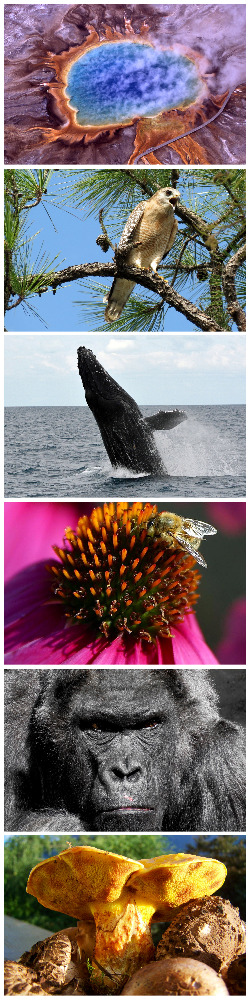
\includegraphics[width=\linewidth]{graphics/diversity-composite.jpg}
\caption{The diversity of life. All images taken from the public domain.}
\label{fig:diversity}
\end{marginfigure}

Is biological evolution a story of progress--is life moving towards a goal, or at least steadily “improving” in some sense? If so, what drives this directional change, given that natural selection does not strive towards any macro-evolutionary goal? If not, why do humans intuitively perceive an evolutionary trend of increasing complexity?

Section \ref{arrow:contingency} examines the null hypothesis: that evolution is a random walk through the possibilities of biology (Figure). In this view, evolution is historically contingent, a series of unpredictable events that appear to show movement towards a goal only in retrospective human perception. The only true movement is a towards a better functional fit to the opportunities and constraints of environment. % Some kind of figure here and for the bottom two here would be nice. Possibly a shifting possibility landscape, with random walks tending to "easier" terrain...but may confuse with fitness landscapes later.

It’s hard not to conclude, however, that life on Earth exhibits a trend of increasing complexity, defined in terms of either genetic information or functional ability. % Evaluate the latter part of this statement after having reviewed the increasing complexity lit.
Section \ref{arrow:complexity} asks whether such a trend, given enough time and partially constrained by physical and chemical forces, could indeed be produced by a passive random walk, or whether a more active generating force is needed. % After lit review, add sentence on complexity theory splitting the difference: a “passive” self-organization. Or perhaps not characterized as splitting the difference.

Section \ref{arrow:cooperation} then introduces the main theme of this book: cooperation. The most revolutionary leaps in evolution—-what biologists call “the major transitions”—-share a common characteristic: each leap allowed previously separate entities to integrate into a new type of individual, a cooperative superorganism. The trend in complexity observed by humans could thus be interpreted as a movement towards more sophisticated forms of cooperation. 



B.3  Contingent versus favored leaps


Contingency can probably be rejected for the first transition, the rise of the hypercycle (Knoll and Wambach, 2000[ Is this true? Why is gene duplication and specialization/lateral transfer so different than anything else?]).

Inherent tendency is a slightly weaker formulation than inherent ‘purpose.’ Such a tendency could be explained by physical, chemical, or biological constraints.  With respect to cooperation, this presumes a lower bound value for a given trait within a clade. Brownian motion is then sufficient to push the trait value upward over evolutionary time (McShea, 1994). 
Various tests for the source of evolutionary change over time are possible (McShea, 1994).
Another important question is the level at which the trend is observed. Molecular evolution, for example, could be broadly deterministic, even while morphological or ecosystem change is contingent (Knoll and Wambach, 2000).

The integration of previously separate organisms may help overcome barriers to evolvability (Futuyma and Kirkpatrick, 2017). A particular physical-chemical arrangement may be stuck on a local optimum. Integration may ‘transport’ the new organism to an entirely different region of the fitness landscape.

The two symbioses that characterize eukaryotic life probably arose as singular events. This suggests that the innovation arose rarely, or that its appearance was so spectacularly successful that it overwhelmed competing strategies,[ Maybe. Even in this case, why wouldn’t it arise in other lineages?] or both.  Multicellularity, meanwhile, has arisen more than ten times in separate lineages (Buss 1987, from Knoll and Wambach 2000), suggesting that it was physically or chemically favored. 

If our view of a small set of powerful and clearly identifiable transitions is correct, than it’s possible that “mini-walls” exist on the metaphorical right side of evolution—barriers occasionally surmounted by a radical innovation (Sterelny 1999; Sterelny and Griffiths 1999, from Knoll and Wambach 2000). It’s not clear, however, whether such walls can be identified a priori, or whether their existence only becomes apparent after the fact. If the latter is closer to the truth, then the “right wall hypothesis” is difficult to confirm or refute.

It’s possible that contingent transitions can give rise to driven trends, or vice-versa. For example, the eukaryotic symbiosis between mitochondria and an ancient archaeon—probably a singular event—permitted the transition to multicellularity. Multicellularity itself led to new biological resources becoming available to be metabolized by other organisms (Knoll and Wambach, 2000). 

Contingency can also foreclose potential pathways of evolution. Bacteria, while having evolved an impressive array of metabolic strategies, appear to lack the capability to diversify in terms of replication…[or other eukaryotic traits?]. This is possibly because their metabolic mechanisms rely on the diffusion of various [substrates, oxidants, and reductants] into cell interiors, which imposes limits on cell size (Knoll and Wambach, 2000). Small cell size prevents the importation of foreign particles[ is this the reason? check K and W]…and also constraints the development of the uniquely versatile inner structure of eukaryotes, including membranes and a flexible cytoskeleton. These traits would allow the evolution of photosynthesis[ though some bacteria can photosynthesize], herbivory, and predation (Knoll and Wambach, 2000). 

Contingency and driven trends are not mutually exclusively. If we accept the right wall hypothesis, random exploration results in an increase in variance around the previous transition. A leap can surmount the right wall, opening the floodgates for more innovation. 

“Mass extinction is generally considered to frustrate selection-mediated evolutionary tra- jectories, but it may also contribute to them via selectivity, the breakdown of ecological in- cumbency, or both” [investigate this more, from Knoll and Wambach, 2000]



[Have major transitions broken down?]

\subsubsection{Contingency}\label{arrow:contingency}

Orthogenesis is the hypothesis that evolution has a direction—that the historical pattern of variations in the genetic code proceed towards a goal, typically by an increase in a particular trait or characteristic (e.g., intelligence). At the other extreme is the notion of contingent evolution, which argues that the trajectory of life is highly sensitive to the influence of singular, unpredictable events. Most biologists hold a view somewhere in between, but almost everyone agrees that  contingency plays an powerful role in various aspects of evolution (Futuyma and Kirkpatrick 2017[ Probably too general of a reference…]). 

Mutation, the ultimate source of genetic variation, is random[ Evaluate—is mutation directed in any sense?]…

Genetic drift has clearly played a determinative role in steering evolution. This is most clearly seen when considering the effects of natural disasters on evolution. 


2. Gould and his examples…
The late Stephen Jay Gould was evolutionary biology’s best-known advocate of the determinative influence of contingency. 
Contingency clearly affects the evolution of traits. Life on earth has at numerous times been greatly reduced by natural catastrophe…Natural selection works within the confines of these disasters. Thus trends may exist over time scales shorter than the entire expanse of evolutionary time. 



 Natural selection itself responds to a fluctuating environment, and has no mechanism to guide macroevolutionary trends. But natural selection is a powerful tool by which to search the biological design space. Given enough time, it will tend to produce forms of higher complexity, which is what we observe in the evolutionary record. 
 
3. Drunkard’s walk—how randomness produces trends. 
Gould famously used the metaphor of a drunkard walking along a wall (Figure ). The presence of the wall on one side ensures that, given enough time, the drunk falls in the gutter. The idea is that any trends we observe in macroevolution are the result of diffusion away from a starting point, a lower bound. A random walk away from the starting point is sufficient for greater and greater complexity (or any other trend) (Gould 1996, from Knoll and Wambach 2000). 
4. Passive vs active trends.
This is the “passive” or “diffusive” view of macroevolution. 
In contrast, “driven” models emphasize an underlying tendency propelling evolution. 
5. The filling of ecospaces.

Macroevolution can also be seen as the gradually filling of ecospace, the full set of ecological niches available for life (Knoll and Wambach, 2000). This shifts attention away from the genome and towards the environment. 

The evolutionary record strongly supports such a reading of history. Knoll and Wambach (2000) identify five “megatrajectories” that mark the filling of global ecospace: 1) the origins of life to the last universal common ancestor (LUCA) of today’s species; 2) the development of metabolic diversity among microbes; 3) endosymbiosis; 4) the movement from aquatic to terrestrial habitats; and 4) human technological progress. 

The idea of ecospace filling is compatible with the notion of trends in complexity, cooperation, or other features. It’s possible that major transitions enable new regions of the ecospace to be explored (Knoll and Wambach 2000). 

The colonization of land is perhaps the clearest example of ecospace filling…

We clearly see a gradual filling of ecospace in the evolutionary history of vascular plants. Innovations like roots, leaves, and wood enabled exploration of new habitats (Knoll and Wambach, 2000). 
6. Ecospace change/env evo

It may also be possible that the environment itself exhibits a trend—that is, environmental conditions are changing in a manner that rewards greater cooperation. Selection then drives the evolutionary increase in cooperative behavior.  This is called a driven trend. 
[Oxygenation, geo-atmospheric/ecological linkages…; microbial diversity as air and ocean oxygenated]
If the environment has indeed changed directionally, then life would be pulled along the trend…(Knoll and Wambach, 2000)
If we think of ecosystem complexity as the density of interactions between species and trophic levels, then macroevolution does show a trend. [From Knoll and Wambach 2000; investigate if such a trend actually exists, and how ecosystem complexity is defined] 
Ecospace filling is limited by physical and chemical constraints.
7. The fitness landscape/the biological design space.

8. How to distinguish passive vs. active.
Irreversibility could serve as a way to distinguish random from driven trends. By definition, random movement on the fitness landscape can be increasing or decreasing in fitness, unless downward movement is prevented by some mechanism. This appears to be the case with endosymbiosis and multicellularity, for example: no eukaryotic lineage has produced prokaryotic descendants, and no multicellular lineage has reverted to unicellularity[ With the exception of myxozoans] (Knoll and Wambach, 2000)



\subsubsection{Complexity}\label{arrow:complexity}

orthogenesis
In the presence of a left wall and a random exploration of the right boundary, we would observe the same outcomes as a driven trend towards complexity would show: greater and greater sophistication. 
For prokaryotes, the left wall may simply be a volume restriction: a certain size is needed to contain the genomic information required for replication, metabolism, and other cellular functions (Knoll and Wambach, 2000)

Box: the fitness landscape
Complexity is not a universal trend (Futuyma and Kirkpatrick, 2017)…many taxa have not evolved considerably in millions of years—sometimes hundreds of millions of years, as in the case of crocodiles[ REF].
The upper bound of cellular complexity is clearly increasing. With complexity comes increased specialization and efficiency (Knoll and Wambach 2000). 
“high-energy species predictably replacing those with lower metabolic requirement” [from Knoll and Wambach, summarizing Vermeij (1999)—investigate]
Complexity can also be defined in terms of the information content of a genome. Unfortunately, quantifying genomic information is not as easy as simply counting the possible combinations of four nucleotides over a genome of a given length, for two reasons. First, the same nucleotide sequence can code for different proteins, through a technique called alternative splicing in which the RNA spliceosome arranges chunks of nucleotides in different orders (Figure X). Second, a given nucleotide sequence can have effects on the expression of genes far away on the chromosome[ genome?]…[multiple binding sites for different transcription factors; others]

The evolution of multicellularity consequently created an ecosystem divisible into trophic levels, which then may have permitted further transitions…[how?] (Knoll and Wambach, 2000). For example, predator-prey evolutionary arms races may have lead to the rise of complex mutualisms, for example between angiosperms and pollinator insects (Knoll and Wambach, 2000[ more details on the link here]). 


	1	C.1	Life as negative entropy
	2	Cooperation as a particularly effective anti-entropic strategy 
	3	
	A.	Biological efficiency is usually described in terms of fitness, but the idea of efficiency as relating to thermodynamic constraints (discussed further in Section 1.C) sheds light on why

C.1 Life as negative entropy

Life is an eddy of negative entropy; genetic replication as a dissipative? self-organized strategy for immortality.

[Eric Smith, non-equilibrium physics; biosphere as far-from-equilibrium system]

Lane 2015

“…the fundamental properties of life necessarily emerged from the disequilibrium of a restless planet”

Photosynthesis: using energy of light “to strip electrons from an unwilling donor”

3.2 GA, life extracting electrons from “almost everything else. Life…is nothing but an electron looking for a place to rest.” (Szent-Györgui)


Cooperation and entropy

C.1 Life as negative entropy

Life is an eddy of negative entropy; genetic replication as a dissipative? self-organized strategy for immortality.

[Eric Smith, non-equilibrium physics; biosphere as far-from-equilibrium system]

Lane 2015

“…the fundamental properties of life necessarily emerged from the disequilibrium of a restless planet”

Photosynthesis: using energy of light “to strip electrons from an unwilling donor”

3.2 GA, life extracting electrons from “almost everything else. Life…is nothing but an electron looking for a place to rest.” (Szent-Györgui)


\textbf{Key terms}

Alleles
Evolution
Gene flow
Genetic drift
Mutation
Natural selection


%------------------------------------------------


\chapter{The Origins of Life}\label{ch:origins}

Life arose cooperatively. Understanding how this happened first requires us to distinguish life from non-life, the subject of Chapter 1. Scientists have proposed many definitions of life over the past 150 years, but none have gained widespread acceptance. The boundary between life and non-life remains vague, although life can be broadly said to be an ordered, cellular, metabolizing, replicating system capable of Darwinian evolution (evolution by natural selection). Although some abiotic systems may have one or more of these features, none have all of them; every living organism does. Science does not yet know how living organisms first emerged more from the inorganic environment of primeval Earth more than four billion years ago.

Chapter 2 details some of the leading theories of life's origin. The debate can be roughly split into two camps: replication-first and metabolism-first theories. The strongest versions of genetics-first theories state that replication preceded the other characteristics of life: molecular systems learned how to copy themselves at acceptable fidelity before developing, for example, metabolic capabilities or cellular compartments. Metabolism-first theories state that life began with the creation of metabolic pathways that captured the energy and matter needed for a molecular system to maintain order over time. Less mainstream ideas propose that cells or other features preceded both replication and metabolism. Regardless of which theory is correct, the origin of life involves some kind of cooperative breakthrough. Both replication and metabolism require a cooperative catalytic network comprised of various molecular species. Each molecular species plays a role in catalyzing the production of another species in the network, and this cooperative cycle enables the entire set of molecules to be replicated.

Chapter 3 discusses various hypotheses about the general framework of ancient cooperative catalytic networks, focusing especially on two kinds of cooperative processes: simple copying of complementary gene sequences and autocatalytic sets. Soon after the origin, life most likely passed through an "RNA world" in which ribonucleic acid performed all important cellular functions—replication (information storage, transcription, and translation), metabolism, and the wide array of other necessary enzymatic reactions. This primitive machinery was soon replaced by a more powerful cooperative schema: division of labor between nucleic acids and proteins.

As discussed in Chapter 4, this arrangement is the basis of all cellular life today. However, it is not clear how this partnership arose, stabilized, or spread. Such questions are important gaps in our knowledge of the early evolutionary history of chemical cooperation.
	3.	The origins of life
	A.	What is life?
	A.1.	The efforts to wrestle with definitions (box of various ones), and what each definition allows in terms of science, ie, description and prediction. Critique of the various ones, and a choice of a working definition for this book: bounded system (has membrane) capable of self-propagation (thus requires replication and metabolism) by evolution by natural selection (so some informational content, subject to mutation, that is transmissible). 
	A.2.	The physical and chemical distinctions between life and non-life.
	A.3.	Is the emergence of life likely or unlikely?
	⁃	Conditions of life on early earth
	⁃	The transition between inorganic and organic chemistry
	B.	Theories of the origin
	B.1.	[Pre-theories of spontaneous generation/] Warm little ponds—Darwin, Miller-Urey, Oparin, Haldane; the key challenges—self-organization (is life thermodynamically and chemically favored?);  
	B.2.	Self-organization of protocells: the RNA world. [Transition] Speigelman, Sutherland, Szostak, etc. Are the challenges of spontaneous membrane formation, replication, metabolism met?
	B.3.	The hydrothermal hypothesis. Wachterhauser, Martin, others. Thermodynamically favored. Compelling critiques?
	C.	The fundamental problem of cooperation
	C.1.	The notion of chemical cooperation—defined by “thermodynamically favored”
	C.2.	The hypercycle: cooperative chemical systems
	⁃	Linkage to metabolism
	⁃	Linkage to replication
	⁃	Linkage to membranes	
	
	
	Process:
0. Free write
1. Origins of life course. Then rewrite draft. 
2. Review notes from core books, update rough draft
	- Koonin & Martin 2005
	- Harold, book 
	- Lane 2015
	- Knoll, book
	- Ward & Kirschvink 2015
	- Maynard Smith/Szathmary 1995 (read, notes)
	- “ 1999 (+reread)
	- Futuyma 2017
3. Locate and review key papers, update rough draft
	- Koonin 2003
	- Check other articles in list
4. 2nd tier books, review notes, update draft
	- Mesler & cleaves
	- De Duve
	- Davies
5. 2nd tier articles, locate and review
6. Revise draft, submit.






\section{What is life?}\label{defining-life}

Defining life
The origins of life pose a difficult problem. Various features—growth, reproduction, heredity, homeostasis, metabolism, cells—have all been proposed as essential to the definition of life. A rough consensus exists that life is a self-propagating system that is capable of evolution by natural selection (Joyce, 1994). Various nonliving systems (for example, crystals) can self-propagate, but they do not evolve by natural selection. The ability to adapt is how life maintains negative entropy. 

Natural selection, however, is unlikely to have created the origins of life: there was no hereditary mechanism by which successful variants could be replicated and transmitted to the next generation. The origins of life must thus be chemical. In particular, a series of chemical compounds must have been integrated in a hypercycle, an autocatalytic set of molecules in which one type of molecule catalyzes/produces another, and so on, in a chain. 

The distinction between life and non-life is not always clear. In fact, the evolution of earth is best seen as a biogeochemical process—that is, one in which biological, geological, and chemical changes drive each other, and are in some cases inseparable. The various means by which bacteria, archaea, and plants obtain energy from the environment—sulfate reduction, methanogenesis, chemoautotrophy, and photosynthesis [Box?]—have a strong influence on the chemical composition of the atmosphere, hydrosphere, and lithosphere. 

[Examples here of biogeochemical cycles]

Is life inevitable?

A key question is if the emergence of life is likely or unlikely. That is, do the origins of life require very narrow chemical and geophysical conditions, and thus would occur very rarely, or does life emerges easily under a range of environmental conditions? For decades, the assumption was the latter, mostly based on the notion that all present life appears to have descended from a common ancestor; that is, life arose only once. Recent years have called this logic into question, for two major reasons. First, nearly all very old rock samples contain evidence of life (Bell et al. 2015; possibly small box with photo), including some over four billion years old. If life were rare, we would except some of these ancient rocks to be devoid of life. Second, as Darwin himself postulated, any independent emergence of life may be quickly consumed by other life that is already present. 

Ironically, the ultimate origin of species is a topic about which Darwin did not write a great deal. In a letter to the eminent biologist J.D. Hooker, he wrote of a “warm little pond, with all sorts of ammonia and phosphoric salts, light, heat, electricity, etc., present, that a protein compound was chemically formed ready to undergo still more complex changes.” The “warm little pond” view of the origins of life held a central place in theorizing for over a century…[Miller-Urey, Spiegelman experiments]

The conditions of early Earth

Did the conditions of early Earth suggest a viable pathway for the emergence of life? The atmosphere was mostly comprised of carbon dioxide, water vapor, nitrogen, and sulfur dioxide expelled from volcanos. 	

\section{Theories of the origin}\label{origin-theories}

The transition from non-life to life is an old subject of inquiry, under the heading of spontaneous generation (Mesler & Cleaves 2016, xvii). 

The building blocks of life

[The arrival/spontaneous production of amino acids]

The problem is essentially one of sequence. A series of experiments over the past half-century, beginning with the famous Miller-Urëy experiments of 1953, suggest that lightning in the early stages of Earth may, in the presence of certain gases, produce amino acids. The atmosphere of the early Earth was largely made of oxidized gases, especially carbon dioxide, water vapor, nitrogen, and sulfur dioxide (Lane 2015).

Others argue that amino acids and other organic molecules may have been carried to Earth by asteroids or as interplanetary dust (Chyba and Sagan 1992). Enormous amounts of organic molecules are present in space (Mesler & Cleaves 2016, 220; seek more information).
	i


….or synthesized from hydrothermal vents. 



[Concentration & functional organization; when does selection start?]

Whichever theory is correct, the basic building blocks of life are not difficult to generate. In the words of the biochemist Nick Lane, “the fundamental properties of life necessarily emerged from the disequilibrium of a restless planet” (Lane 2015, 13). 

More difficult is what comes next: concentrating these molecules in such a way that permits metabolism and replication. The creation of life depends not just on the presence of building materials, but arranging those materials into a functional system—a machine to convert the free energy of early Earth into an oasis of biological order.  

Life requires three characteristics. First, molecules must have been contained with a semi-permeable boundary—that is, the cell must have come into existence. The boundary must permit resources from the outside environment to enter across the membrane, while selectively excluding parasites and preventing cellular components from diffusing outside the cell. 

Second, energy from the external environment (that is, outside the boundary) must have been able to be absorbed through the boundary.

Third, the system must have been able to be replicated. Once these conditions were in place, natural selection would be able to drive biological evolution. 

The problem is that it is difficult to imagine these conditions arising without natural selection already being in place. An entity as complex as a metabolizing, replicating cell is unlikely to have arisen by means other than natural selection. In addition, the order in which cells, metabolism, and replication arose is not clear. Cells would not seem to confer a fitness advantage if they could not metabolize and replicate. The energetic gains of metabolism would dissipate without a cellular boundary, and a metabolic innovations would quickly be lost without replication machinery. Replication is meaningless without a cellular boundary—there would be no cohesive unit to evolve together—and probably impossible without the ability to metabolize resources.

The classical debate was between the “metabolism first” advocates, led by Oparin, and the “replication first” school, led by JBS Haldane (Mesler and Cleaves 2016, 144). Metabolism-focused theories suggest that something with the functional power of proteins evolved first…Replication-based theories, on the other hand, argue that an RNA molecule, or something like it, came first (Mesler and Cleaves 2016, 195). 

Two broad families of theories, centering on protocells and ?, have been proposed to explain this puzzle.

Protocells and the RNA world

First, some suggest that protocells—able to metabolize and possessing some kind of primitive membrane, but not able to replicate in the way that current cells do, through the genetic code—organized spontaneously (Shenhav et al. 2003, Walker and Davies 2003, Szostak et al. 2001, Deacon and Sherman 2007) (Figure).  This assumes that such a design did not require natural selection, and instead was made probable by tendencies of self-organization. 

The ‘RNA world’ body of ideas falls into this category.

This initial molecule did all the work that DNA, RNA, and proteins do now. 

A present-day membrane-enchased RNA molecule that metabolizes and replicates has thus far not been found (Mesler and Cleaves 2016, 250). 

The problem is that long sequences of RNA would have a high mutation rate, and thus accurate replication would be difficult (Futuyma and Kirkpatrick 2017, 437). 

In recent years some studies have shown that the process of self-assembly from free-floating molecules to RNA is possible (CHECK SUTHERLAND), and have also outlined the possible steps by which proto-RNA could have obtained a lipid membrane (Szostak, from Zimmer) and the ability to replicate (Lincoln & Joyce, from Zimmer) . The transition from an RNA world to the present DNA/RNA configuration is an easier leap (see [later part of this chapter? Next chapter?]). 

Second, some postulate the spontaneous creation of a simple precellular structure that separated itself from the environment by means other than the kind of barrier that life has today, a lipid-based membrane. These rudimentary cells could replicate roughly accurately as daughters inherit parental stoichometry (Baum 2015) (Figure). This pushes the role of selection back a fit further, but still demands that a cell-like structure must have arisen without the influence of natural selection. Aerosol droplets, cavities in porous rocks, clay crystals, and aggregations held together by internal chemical interactions have all been proposed as possible versions of this “precell” (Dobson et al. 2000; Kuhn and Waser 1981; Cairns-Smith 1966, 1990; Oparin 1957, Fox 1988) [from Baum 2015]). 

[The hydrothermal hypothesis]

Finally, some theories hypothesize that selection was active at an even earlier stage (Wachterhauser 1988, 1990, 2007; Pross 2012; others). 



[CLARIFY WACHTERHAUSER hypothesis: two-dimension origin, mineral surfaces; primitive metabolism; CO2 reduced by H2S.] These molecules have not clearly been shown to be auto-catalyzing, however…(SEE orgel 2000; https://www.ncbi.nlm.nih.gov/pmc/articles/PMC18793/)
	
…

Molecules on a rock surface catalyzed each other in a hypercycle (Figure). Neighborhoods of autocatalytic units—initially overlapping and indistinct, unbounded by a barrier—participated in a primitive form of metabolism and replication. Without a membrane and template replication machinery, these aggregations of free protoplasm were likely highly unstable. Selection, however, could have acted on these neighborhood hypercycles even in the absence of a membrane. 

The current leading theory of the origins of life postulates that inorganic rock-like compartments in hydrothermal vents provided the analog of a cellular boundary. Energy from the vents, in hydrogen form, powered the hypercycle. The molecular system that were able to replicate themselves most successfully proliferated. At some point, a system created an RNA-based technique of encoding its structure in a sequence of nucleotides. This system proved so successful at replicating that it quickly outcompeted the other variants. Eventually, a division of labor between DNA and RNA proved even more efficient. 

The hydrothermal theories revive the metabolism-first school. Life began as a hypercycle inside cell-like rocky compartments, feeding on carbon dioxide and hydrogen sulfide. Instead of cell membranes, sulfide bubbles segregated outside and inside (Russell and Hall, from Wachterhauser and Mesler/Cleaves 2016, 238).

In some versions of the theory, selection for the ability to colonize new surfaces—that is, to travel—led to the encasement of these cooperative metabolic cycles within propagule-like structures (Baum 2015) (Figure). Selection would have acted more forcefully on these cellular bodies, leading to improvements in metabolism and the replication machinery.  “…cellular life is composed of heterogeneous chemical moieties that cooperate to generate more of the same” (Baum, 2015). Mobility also allows the propagule to harvest energy and metabolites available in the water column (Baum, 2015). 


Wachterhauser argues that the substrate was iron pyrite, on which organic molecules used redox potential energy to fix carbon, allowing growth and replication. 

Martin and Russell (2007; ) suggest that warm alkaline vents would have provided the requisite energy flow and mineral superstructure, and allowed the evolution of electron transport chains across membranes. The underwater habitat would have shielded nascent life from damaging ultraviolet radiation (Martin and Russell 2007). 

In their view, H2 from hydrothermal vents reacts with dissolved carbon dioxide in the oceans, providing a chemical energy source. The vents themselves provide a cell-like microporous structure that concentrates organic molecules without the need for a lipid membrane. Such a scenario is thermodynamically favored: instead of organic molecules needing to fight entropy…[explain how favored]

This last family of ideas requires only chemical building blocks, free energy, and a mineral medium on which to grow for life to arise. Selection does the rest, taking the burden off random chance. The great advantage of this theory is that it allows selection a role before the emergence of any kind of bounded entity (Baum 2015), which reduces the reliance on chance events. Selection comes before the cell, instead of the other way around (Baum, 2015). 

\section{Chemical cooperation: catalytic networks}\label{chem-coop}



The hypercycle & chemical cooperation

Cells represent the creation of individual ‘selves.’ The membrane represents a contract between the various components of the hypercycle in the struggle for existence. The contract specifies the terms under which key collective functions—especially the common defense, control of internal cheating, and the general division of labor for coordinated activities like uptake and metabolism of resources—are carried out.

The hypercycle presents one possible solution to the problem of faithfully replicating…

Is this the interaction between molecules cooperative? We return to a possible definition of cooperation as behavior between two or more entities that provides mutual benefit—and eventually leads to mutual obligate dependence. Catalysis is one possible form of cooperation; the hypercycle represents a network of mutual dependence. Molecules, in isolation, are not living entities. There is no clear line of demarcation between what is living and what is not. But the process of cooperation, the possibility of endless catalysis and replication into the indefinite future, gets us closer to the intuitive notion of life as something that actively sustains itself by interacting with its environment. Life will likely never be defined precisely, but cooperation appears to be essential to something fitting the intuitive definition. 

In the initial phase of life, those chemical molecules which could cooperate within hypercycles replicated at greater frequencies—with adequate accuracy—than those chemicals that did not cooperate. This is the fundamental pattern that’s repeated throughout all of the major transitions. A new kind of individual was created, a new system to serve as the target of selection. 

Neighborhoods are a contingent circumstance in order to promote creation of hypercycles: the right chemicals—the combinations required to initiate and sustain a hypercycle—must be present in sufficient quantities in a given local area. Thus the specific nature of the adsorbing mineral surface is important. Contingent neighborhoods become “cooperative autocatalytic neighborhoods” (Baum, 2015). 

There is no easy way to fundamentally distinguish life from non-life. This complicates our notion of cooperation—and any form of interaction, including predation and parasitism. Nick Lane has remarked that “all kinds of life parasitize the environment.” (P55, 2015).

Life has profoundly influenced Earth’s geochemical cycles….Great Oxidation Event…Bacteria are responsible for the creation of [a great deal of] sedimentary rocks (Lan	e 2015). 

We may never possess a narrow and precise definition of life. We do not know whether our current definitions are too narrow—that is, whether life could be non-cellular, non-carbon-based, or exist in other forms. 

Regardless of which theory best explains the origins of life, chemical cooperation will play a critical role. The creation of hypercycles—molecular partnerships that increase the efficiency of metabolism and replication—appears to be an essential stage in any theory. If complexity is the converse of entropy—the presence of more functional modules, the presence of more fine-grained, information-rich order—then cooperation is the means to arriving at complexity. Complexity does not increase by chance (Baum, 2015)

Possible: 

Group selection in a 2D array, without boundaries [check Grim et al. 2006]

\section{Nucleic acid-protein cooperation}

Nucleic acids and proteins have quite different chemical requirements. High-fidelity replication of nucleic acids requires a one-dimensional transcription system with very little reactivity, while the catalytic action of proteins depends on highly reactive, three-dimensional changes (Ruiz-Mirazo et al. 2004). "Partly decoupled but strongly complementary"

Lewontin, from Tsokolov: "DNA is a dead molecule, among the most non- reactive, chemically inert molecules in the world.... The linear sequence of nucleotides in DNA is used by the ma- chinery of the cell to determine what sequence of amino acids is to be built into a protein, and to determine when and where the protein is to be made’’



% May want to broaden or narrow this heading/section subject


%----------------------------------------------------------------------------------------
\chapter{The Genome}\label{ch:genome}

5

Molecular cooperation: replicating genomes


Genomes are cooperative enterprises: genes working together to optimize the inclusive fitness of the individual in which they are housed. As do all biological entities, each gene tries to maximize the benefits of cooperation while minimizing its costs, in some cases adapting strategies to replicate itself in the next generation at higher than ‘fair’ frequencies. The ‘social contract’ between genes is thus always under stress by potential cheaters, and this tension between cooperation and cheating has molded, through evolutionary time, the structure of modern genomes. Cheating has not, though, arrested the general trend of evolution, which points towards greater genomic cooperation, with increasingly specialized genes exchanging information and dividing labor within sophisticated network architectures.

This chapter looks at molecular cooperation within the cells of living organisms, with the molecules of interest being the nucleotide bases that make up the genome. Section 4.1 briefly describes the genetic machinery within each cell. Section 4.2 then looks at the structure of gene cooperation, especially regulatory networks and the meiotic process of assuring ‘fair’ replication into the next generation. Section 4.3 outlines the various cheating strategies that genes employ, and how the use of these strategies over billions of years explains the puzzling structure of modern genomes. Section 4.4 looks at the arrow of genomic evolution, with a special focus on the origins of life, and discusses proposals for measuring the magnitude of genomic cooperation.

- Discuss the difficulty of defining a ‘gene,’ and why “molecular cooperation” instead of “genomic cooperation”
- Horizontal gene transfer


Lane 2015

Adaptation: everything goes. “Genomes recall the past: they reflect the exigencies of history.”


\section{The fundamentals of cellular genetics}\label{cell-genetics}

4.1	 The fundamentals of cellular genetics

Life is encoded in deoxyribonucleic acid (DNA), a molecule arranged in the shape of a double helix and stored inside the nucleus of each cell of an organism’s body. DNA is made of smaller molecular units called nucleotides, each of which contains the sugar deoxyribose, a phosphate group, and one of four nitrogenous bases: adenine (A), cytosine (C), guanine (G), and thymine (T). The nucleotides are arranged in pairs, A-T and C-G, along the two strands of the helix (Figure, DNA). Each string of three nucleotides is called a codon. Each of the unique 4tothe3 (64) codons is a sign representing one of 20 amino acids, with substantial repetitions and three codons signifying a ‘stop’ signal (Figure, genetic code). A sequence of codons are transcribed from DNA by messenger ribonucleic acid (mRNA) and then transported to the ribosome, the cellular structure responsible for making proteins. Within the ribosome, transfer RNA (tRNA) translates each codon in the sequence as its associated amino acid (or stop signal). The chains of amino acids are known as proteins, the molecules that perform the various functions of the organism’s body (Figure, cellular machinery). 

A gene is conventionally defined as the nucleotide sequence used to create a protein molecule. The story is more complex, however. The coding regions of genes are called exons, but these comprise only a small fraction of the overall genome—perhaps 5% of the human genome, for example (REF). Interspersed with exons are introns, non-coding nucleotides that are not transcribed but rather spliced out before mRNA transcription. Surrounding the gene are enhancers and repressor nucleotides that bind transcription factors, proteins created by other genes that control whether transcription occurs, as well as promotors that bind the mRNA molecule. In addition, large parts of the genome—nearly half in humans—appears to be made up of repeated sequences, which were likely formed by genes copying themselves in the past, a processed called transposition. These transposable elements (TEs) strongly hint at extensive cheating within the genome, an issue taken up in Section 5.3.

This complicated picture has become even muddier in recent years. The discovery of gene regulatory networks (GRNs) suggests that the transcription of certain genes depends on nucleotide sequences located faraway on the genome, and exons from different genes can be part of the same transcribed mRNA…in addition, the mRNA itself than remove some of the coding regions during transcription, a process called alternative splicing. Thus the same transcribed sequence can produce different proteins…These issues are discussed in more detail in Section 5.2.


Evolution of genomes? Viral and transposable elements here?


\section{Genomic networks}\label{gene-net}

	5.2.1	Gene regulatory networks

	5.2.2	Meiosis as fairness mechanism

\section{Transposons}\label{transposons}

Transposable elements

\section{Horizontal gene transfer}
Horizontal gene transfer
    Transduction, transformation, conjugation
    
\section{Cellularization and individuality}

% Also could call 'cheating genes'



%----------------------------------------------------------------------------------------

\chapter{Endosymbiosis}\label{ch:endosymbiosis}

From Knoll and Wambach, 2000: “Martin and Muller (1998; see also Moreira and Lopez-Garcia 1998) have proposed that the domain originated via an ur-symbiosis be- tween a facultatively anaerobic proteobacter- ium that fermented organic molecules to hy- drogen and carbon dioxide and an archaean (possibly methanogenic) able to metabolize these waste products”


Lane 2015
-Life began 4 GA, but stuck at bacterial level for 2b years. Big gap between bacterial complexity and eukaryotic complexity


\section{Mitochondria}\label{mitochondria}

\section{Chloroplasts}\label{chloroplast}

\section{Sociovirology}\label{socioviro}

Munoz-Diaz, West


Brosius J (2003) The contribution of RNAs and retroposition to evolutionary novelties. Genetica 118:99–116

Forterre P, Prangishvili D (2009) The great billion-year war between ribosome- and capsid-encoding organisms
(cells and viruses) as the major source of evolutionary novelties. Proc NY Acad Sci, 1178:65–77

% Possibly fits better elsewhere, or in a compact (not full section) format



%----------------------------------------------------------------------------------------

\chapter{Multicellularity}\label{ch:multicell}

“Gene expression became regulated by molecular signals transduced from a cellular rather than physical environment to produce multicellular organisms characterized by ontogenetic cell differentiation” 

“-Multicel- lular organisms diversified in a third distinct way: via the functional integration of cells me- diated by development”

(Knoll and Wambach, 2000)

Lane 2015

30 separate origins of multicellularity 

Specialization

Colonial life (man o’war, aspens, slime molds, corals)

The organismality debate



%----------------------------------------------------------------------------------------

\chapter{Sex and Cooperative Recombination}\label{ch:sex}




%----------------------------------------------------------------------------------------

\chapter{Parental Care}\label{ch:parenting}


(Parental care is kin selection), way of introducing this?




%----------------------------------------------------------------------------------------

\chapter{Eusociality}\label{ch:eusociality}


Eusociality evolves only under certain conditions: where offspring do not disperse away from the parental habitat, reproduction is either asexual or partners are strictly monogamous over a lifetime (West et al., 2015). 


%----------------------------------------------------------------------------------------

\chapter{Coordination and Reciprocity}\label{ch:coord-recip}

Chapter 6. Organismal cooperation: kin selection, coordination, and reciprocal altruism
Discussion of kin selection through examining the evolution, genetics, and behavior of eusocial species, especially social insects. A population genetics-based analysis of the costs and benefits of eusociality, with a detailed analysis of adaptations for sanctioning cheating. Detailed examination of reproductive division of labor, cooperative brood care, and intergenerational social life. Discussion of various forms of cooperation among non-related individuals, including cooperative breeding and alloparenting, grooming and cleaning behavior, group hunting, alarm calls, and food sharing. 


Sex
Parental care
Kin selection
Eusociality
Inclusive fitness

[Definition of eusociality]

The social insects have been extraordinarily successful. Once cooperation takes hold, it doesn’t let go: termites have been around for over two hundred million years, ants 150 million, bees 70 to 80 million. Compare this with the typical historical span of a species…Before humans, the typical life of a mammalian species was a mere five hundred thousand years. Eusociality may have come to entirely dominate Earth, but evolution takes place slowly enough to allow other species to adapt (Wilson 2012, 15). The current anthropogenic extinction is an exception: human social systems have evolved so rapidly that biological evolution cannot keep pace. 

Eusociality requires the next generation to stay in the home colony rather than dispersing (Wilson 2012, 141), and for conditions that incentivize a division of labor (Wilson 2012, 153). The environment is thus the fundamental catalyst for eusocial life.

Eusociality can be thought of in the ‘extended phenotype’ formulation of Richard Dawkins (1982). Workers in a bee colony, for example, are “ambulatory parts of [the queen’s] phenotype” (Wilson 2012, 143).

Only a single beetle species is eusocial (Wilson 149, 2012). 

Eusociality is uncorrelated with brain size (Wilson 2012, 39).

Nest defense is a driving force in the evolution of organismal cooperation (Wilson 2012, 17).

A wide variety of mammalian species are cooperative hunters: chimpanzees, capuchin monkeys, lions, wolves, wild dogs, naked mole rats, Damaraland mole rats…(Wilson 2012, 40).

Signaling
Signaling can sometimes be deceptive…
If both parties realize benefits to cooperation, then honest signaling will be selected. In some cases, signals are complex and costly enough that they cannot or will not be faked (West et al., 2015). 

Preadaptations to optimizing fitness benefits of cooperation
Eusociality may require pre-adaptations for its full benefits to be realized. In the case of humans, key pre-adaptations included body size, prehensile hands, bipedalism, an omnivorous diet, and the use of fire (Wilson 2012, 46).

Eusociality among mammals
The naked mole rat…


\section{Cooperative breeding, grooming, and protection}\label{coop-breeding}

\section{Behavioral coordination}\label{coordination}

\section{Reciprocal altruism}\label{reciprocity}


%----------------------------------------------------------------------------------------

\chapter{Mutualisms}\label{ch:mutualism}

“The metabolic products of one organism pro- vide substrates for another, with the conse- quence that metabolic innovation can fuel di- versification throughout a community. The re- dox complementarity of microbial metabo- lisms further ensures that materials will be cycled among environments as well as among organisms.” (Knoll and Wambach, 2000)


\section{Mycorrhizal networks}

\section{Pollination}

\section{The human microbiome}

\section{Superorganism theories}

Gaia

One bacterial organism



%----------------------------------------------------------------------------------------

\chapter{Human Social Cooperation}\label{ch:social-coop}

\section{Gene-culture co-evolution}

Evolution is fundamentally historical. Much of the pushback against evolutionary theory as the basis for understanding human history and human destiny comes from the notion that natural selection is so powerful and determinate that humans have little scope to manage their affairs…that human society trudges on, believing itself to be in command of its destiny, but in reality insensate to the blind watchmaker that designs the mechanism. 
But there are two satisfactory ripostes to this. First, insofar as natural selection is a law, it is a statistical law.  Disasters and other chance events lead to genetic drift, the random appearance and disappearance of alleles in a population. Migration and mutation also influence the gene pool. So selection operates on a population, but its power for a given population at a given time is unknown. Second, selection cannot be predictive without a knowledge of how the environment will change. 


A few million years ago, it would not have been clear that human beings were the only social species that could have come dominate the earth (Wilson 2012, 49). But the chances are great that it would have been some social species…


If we looked upon the planet a few million years ago, we might have not have bet on primate, or hominid, lines to dominate the Earth. The chances are great, however, that some social species would rise. That position is the great hope of evolutionary prediction: that biological entities do self-organize in some fundamental way, and cooperation is the strategy that, chaos and contingency notwithstanding, eventually wins. 

If such evolutionary principles are general—if they apply with equal force to human as non-human biological systems—then 

Of course, chaos and contingency do matter… 

Among humans, the sharing of goals and intentions—powerfully facilitated by language—is central to cooperation (Wilson 21012, 226). 

It is not clear what drove the Great Leap Forward. Genetic mutations for syntactical language and abstract thought, environmental change, and…are leading theories (Wilson 2012, 85; 217). Language not only communicates information, but creates a relationship between the communicants (Wilson 2012, 230).

Which mutations could have enabled the capacity for language? [Investigate…]

Mutational change in humans is thought to have been low and steady up until about 50,000 years ago, around the time of the GLF, peaking at the dawn of the Holocene about 10,000 years ago. Nearly one-tenth of the amino acid changes since the divergence of humans and chimpanzees four million years ago are thought to be adaptive, an oddly high figure…(Wilson 2012, 87; check Gojobori et al PNAS 2007).



Gene-culture co-evolution

Lactase production was enabled by four independent mutations, three arising in Africa and one in Europe (Wilson 2012, 198).


Social norms
Cooperation is expressed clearly in cultural terms by the ethic of reciprocity. As Rabbi Hillel once remarked, “Don’t do unto others what is repugnant to you. All else is commentary.” (Wilson 2012, 245[ Probably don’t use, too common. Unless in an unconventional fashion]).

Empathy is a fundamental social ability. Empathy assists not only with cooperative action, but also in providing the information necessary for manipulation and deception, which are also quintessential social behaviors (Wilson 2012, 44). The adaptive functions of most human emotion is clear. As Pinker (2002) notes, emotions can be divided into four major categories:
- other-condemning, to punish cheaters: contempt, anger, disgust 
- other-praising, to reward altruists: gratitude, moral awe (being moved) 
- other-suffering, to help needy beneficiary: sympathy, compassion, and empathy 
- self-conscious, to avoid cheating, repair effects: guilt, shame, embarrassment 

Reputation is an important mechanism for incentivizing pro-social behavior. 

Art
Art helps to define group identity (Wilson 2012, 283).



\section{Social norms theory}

\section{Intrahousehold bargaining}

\section{Digital networks}

%----------------------------------------------------------------------------------------

\chapter{Human Economic Cooperation}\label{ch:econ-coop}

\section{Common pool resources}

\section{Club goods}

\section{Pure public goods}

%----------------------------------------------------------------------------------------

\chapter{Human Political Cooperation}\label{ch:poli-coop}

The rise of the state
The first states appeared in the 4th millennium BCE. The Egyptian state rose around 3400 BCE, followed by states in the Indus valley around 2900 BCE…

The Sumerians invented the first writing system around 4400 BCE, with the…independently creating systems of their own…

\section{Social choice theory}

\section{Voting systems}

\section{Legislative systems}

\section{Judicial systems}

%----------------------------------------------------------------------------------------

\chapter{Case Studies: International Cooperation}\label{ch:intl-coop}

\section{The dilemma of global governance}

\section{Climate change}

\section{Infectious disease}

\section{Cross-border violence}

%----------------------------------------------------------------------------------------

\backmatter

%----------------------------------------------------------------------------------------
%	BIBLIOGRAPHY
%----------------------------------------------------------------------------------------

\bibliography{bibliography} % Use the bibliography.bib file for the bibliography
\bibliographystyle{plainnat} % Use the plainnat style of referencing

%----------------------------------------------------------------------------------------

\printindex % Print the index at the very end of the document

\end{document}